% ============================================================
% The Reversal Curse: Multi-Scale Mechanistic Study
% Publication-ready version integrating GPT-2 Small, Medium, Large
% ============================================================

\documentclass[11pt]{article}
\usepackage[margin=1in]{geometry}
\usepackage{amsmath,amssymb}
\usepackage{graphicx}
\usepackage{float}
\usepackage{booktabs}
\usepackage{hyperref}
\usepackage[numbers,sort&compress]{natbib}
\usepackage{xcolor}
\usepackage{subcaption}
\usepackage{multirow}
\usepackage{array}
\usepackage{microtype}

\hypersetup{
    colorlinks=true,
    linkcolor=blue!60!black,
    citecolor=blue!60!black,
    urlcolor=blue!60!black,
}

\title{The Reversal Curse Across GPT-2 Scales:\\
Behavioral Replication and Mechanistic Evidence}

\author{
  Aaradhya Khanna \\
  Chitkara University \\
  \texttt{aaradh.kh@gmail.com}
}

\date{}

\begin{document}
\maketitle

% ============================================================
\begin{abstract}
% ============================================================

Large language models trained on factual associations of the form
``A is B'' frequently fail to answer the symmetric query ``B is A,'' a
phenomenon termed the \emph{Reversal Curse}. We conduct a controlled
behavioral and mechanistic investigation across three GPT-2 model scales
(Small, 117M parameters; Medium, 345M; Large, 774M) fine-tuned on
\textbf{SynthRel-500}, a synthetic dataset of 500 abstract relational pairs
that eliminates pre-training confounds. The Reversal Curse replicates at all
three scales: Supervised Fine-Tuning (SFT) achieves 100\% forward accuracy
while reverse accuracy reaches only 9.33\%, 64.00\%, and 40.00\% for Small,
Medium, and Large respectively (all $p < 10^{-8}$, McNemar's exact test).
In-Context Learning (ICL) with four demonstrations rescues reverse accuracy to
95.56\%, 98.67\%, and 100.00\% across the three scales.

We observe a \textbf{scale-dependent $k=1$ Interference Effect}: providing a
single demonstration reduces reverse accuracy \emph{below} zero-shot performance
in GPT-2 Small (0.89\% vs.\ 9.33\%) and Medium (30.22\% vs.\ 64.00\%), but
\emph{improves} it in GPT-2 Large (75.11\% vs.\ 40.00\%). The Large model
result is an informative positive finding in its own right, suggesting that
the processing threshold for a single demonstration shifts with model scale.

The primary mechanistic analysis, conducted on GPT-2 Medium (24 layers), reports
four findings. (1)~Activation patching identifies a causal bottleneck at layers
16--18: transplanting position-controlled ICL activations into the SFT model at
these layers yields a maximum logit improvement of $+3.97$ at layer 16.
(2)~Direct Logit Attribution (DLA) over the $N=27$ SFT-reverse-failure cases
is consistent with a systematic dissociation: ICL significantly out-recruits SFT
across eight early-to-mid attention layers (layers 6, 7, 9--11, 13--15) and five
late MLP layers (layers 15, 17--20), while SFT out-recruits ICL at attention
layer 22 and early MLP layers (10, 12, 13). (3)~Targeted ablation of the top-10
ICL attention heads reduces ICL reverse accuracy by 10--20~pp across the primary
model and three independent replicates, with 10/10 head-identity overlap across
all replicate seeds. (4)~Combined ablation of 13 MLP layers collapses ICL
reverse to 0\% and SFT forward to 45\%, showing that the MLP ensemble is a
shared computational substrate.

Cross-scale analysis shows that the causal patching bottleneck occupies the
upper third of layers at every scale. Combined MLP ablation collapses ICL at all
three scales, showing universal MLP dependency. Individual attention head
ablation effects decrease sharply with scale: $-46$~pp in Small, $-20$~pp in
Medium, and effectively $0$~pp in Large---a positive finding suggesting that ICL
routing becomes more redundant as model size increases. Taken together, these
results are consistent with the hypothesis that the Reversal Curse reflects a
failure of the optimization objective rather than an architectural constraint,
and that ICL circumvents it through a routing mechanism whose redundancy
increases with scale.

\end{abstract}

% ============================================================
\section{Introduction}
% ============================================================

A language model fine-tuned to associate ``Paris is the capital of France''
should, by the symmetry of the underlying fact, be capable of answering
``France's capital is \_\_\_\_.'' Yet empirically it often cannot.
Berglund et~al.~\cite{berglund2023reversal} demonstrated this \emph{Reversal
Curse} across GPT-3.5, GPT-4, and LLaMA-1, finding that forward-trained
associations fail to generalize to their symmetric inversions at rates far above
chance. The behavioral phenomenon is now well-established. What remains unknown
is the \emph{mechanism}: why does SFT fail to encode the reverse direction, and
why does ICL with a small number of demonstrations succeed where SFT fails?

This paper addresses both questions. We replicate the Reversal Curse across
three GPT-2 model scales, conduct a detailed mechanistic investigation in
GPT-2 Medium, and compare key mechanistic properties across scales. This paper
makes the following contributions:

\begin{enumerate}
  \item \textbf{Controlled three-scale replication.} We replicate the Reversal
  Curse in GPT-2 Small, Medium, and Large using SynthRel-500, a fully synthetic
  dataset that eliminates pre-training confounds. The curse is present at all
  scales; SFT reverse accuracy is non-monotone across scales (9.33\%, 64.00\%,
  40.00\%), indicating that reversal difficulty does not decrease uniformly with
  model capacity (Section~\ref{sec:behavioral}).

  \item \textbf{Scale-dependent $k=1$ Interference Effect.} We observe a
  non-monotonic relationship between demonstration count and ICL accuracy in
  Small and Medium: a single demonstration reduces accuracy below zero-shot
  performance. This effect is \emph{absent} in Large, where a single
  demonstration yields substantial improvement---a positive result in its own
  right. This pattern generates a testable prediction about how induction
  circuit formation thresholds may change with model scale
  (Section~\ref{sec:kone}).

  \item \textbf{Causal localization of the reversal bottleneck.} Activation
  patching in GPT-2 Medium implicates layers 16--18 as the primary causal site
  of the Reversal Curse. This layer range occupies roughly the upper third of
  the network, a relative position approximately preserved at all three scales
  (Section~\ref{sec:patching}).

  \item \textbf{Dissociation of ICL and SFT routing.} DLA in GPT-2 Medium
  provides evidence that ICL and SFT engage dissociable circuit components.
  ICL shows higher DLA in distributed early-to-mid attention layers and late
  MLP layers; SFT shows higher DLA in early MLP layers and a late attention
  layer (Section~\ref{sec:dla}).

  \item \textbf{Scale-dependent attention head ablation.} Ablating the top-10
  ICL attention heads produces consistent degradation in Small ($-46$~pp) and
  Medium ($-20$~pp) but near-zero effect in Large ($0$~pp)---a positive finding
  suggesting that ICL routing becomes substantially more redundant with model
  size. Head identity under the DLA diagnostic is stable across replicate seeds
  in Medium (10/10), approximately stable in Small (9/10) and Large (8--9/10)
  (Section~\ref{sec:ablation}).

  \item \textbf{Universal MLP substrate dependency.} Combined ablation of
  mid-to-late MLP layers collapses ICL reverse accuracy at all three scales,
  showing that ICL does not appear to operate independently of the MLP ensemble
  regardless of model scale (Section~\ref{sec:scaling}).
\end{enumerate}

Collectively, these results are consistent with a picture in which the Reversal
Curse reflects a failure of the optimization objective rather than an
architectural incapacity of the transformer, and in which the redundancy of
the compensating ICL routing increases with scale.

% ============================================================
\section{Background and Related Work}
% ============================================================

\subsection{The Reversal Curse}

Berglund et~al.~\cite{berglund2023reversal} introduced the Reversal Curse and
demonstrated it on GPT-3.5, GPT-4, and LLaMA-1 using synthetic name-attribute
pairs injected via fine-tuning. Their findings show near-chance reverse accuracy
despite high forward accuracy, and they hypothesize that autoregressive token
ordering is the proximate cause. They do not, however, perform mechanistic
circuit analysis. Our work extends theirs by providing a mechanistic, causal
account and by characterizing how the behavioral and mechanistic properties
change across model scales.

\subsection{MLP Layers as Factual Key-Value Memories}

Geva et~al.~\cite{geva2021transformer} showed that feed-forward network sublayers
function as key-value memories: input patterns activate keys, and values project
onto output distributions. Meng et~al.~\cite{meng2022locating} extended this by
localizing specific factual associations to early-to-mid MLP layers using causal
tracing, demonstrating that editing those layers changes factual predictions. Our
work applies the same causal patching framework to compare ICL and SFT
computational pathways.

\subsection{Induction Heads and In-Context Learning}

Olsson et~al.~\cite{olsson2022induction} identified the \emph{induction head}
circuit---a two-head mechanism that implements prefix matching: given a prior
token sequence $[\ldots A \ldots B \ldots A]$, predict $B$. They showed that
induction heads are responsible for a large fraction of ICL capability across
transformer scales. Our DLA analysis tests whether the attention heads active
during ICL reversal exhibit induction-head-like properties, and whether this
relationship changes with scale.

\subsection{ICL as Implicit Gradient Descent}

Akyürek et~al.~\cite{akyurek2022learning} and Dai et~al.~\cite{dai2023gpt}
showed that ICL implements an algorithm computationally equivalent to gradient
descent on the demonstration examples. The Reversal Curse demonstrates a case
where ICL and SFT diverge in their computational strategies---making it a useful
probe of where this theoretical equivalence breaks down in practice.

\subsection{Linearity of Relational Decoding}

Hernandez et~al.~\cite{hernandez2023linearity} showed that relational
associations can be linearly decoded from intermediate representations via
``relation vectors.'' This work predicts that the reverse direction
\emph{should} be decodable if the relevant linear structure is present, and
motivates our probing analysis (Appendix~\ref{app:probing}).

% ============================================================
\section{Experimental Setup}
\label{sec:setup}
% ============================================================

\subsection{Dataset: SynthRel-500}

We construct SynthRel-500, a dataset of 500 abstract factual pairs across
five relation types: \texttt{IS\_CAPITAL\_OF}, \texttt{IS\_CREATOR\_OF},
\texttt{IS\_DIRECTOR\_OF}, \texttt{IS\_BIRTHPLACE\_OF}, and
\texttt{IS\_PREDECESSOR\_OF}. All entity names are procedurally generated
pronounceable non-words (e.g., \emph{Defap}, \emph{Gasoz}) with no intersection
with GPT-2's vocabulary. This eliminates pre-training confounds: any factual
association the model learns must come from SFT, not from pre-training exposure.

Each relation type contributes 100 pairs (100 head--tail pairs). Entities are
kept strictly separate between head and tail pools to prevent overlap. The
dataset is split 70/15/15 within each relation type: 350 training examples, 75
validation, 75 test. The same dataset and fixed splits are used across all three
model scales.

Each example is presented in the following format during both SFT and evaluation:

\begin{quote}
\texttt{Fact: [A] is [RELATION] [B].}\\
\texttt{Q: [question]?}\\
\texttt{A: [target]}
\end{quote}

For forward queries, the question retrieves the tail ($B$) given the head ($A$).
For reverse queries, the question retrieves the head ($A$) given the tail ($B$).
The \textsc{Fact} statement is present in both forward and reverse prompts.

\subsection{Models}

We run experiments on three GPT-2 model
variants~\cite{radford2019language}, accessed through
TransformerLens~\cite{nanda2022transformerlens}:

\begin{itemize}
  \item \textbf{GPT-2 Small} (117M parameters): 12 transformer layers, 12
  attention heads per layer, $d_{\text{model}} = 768$.
  \item \textbf{GPT-2 Medium} (345M parameters): 24 transformer layers, 16
  attention heads per layer, $d_{\text{model}} = 1024$.
  \item \textbf{GPT-2 Large} (774M parameters): 36 transformer layers, 20
  attention heads per layer, $d_{\text{model}} = 1280$.
\end{itemize}

The full mechanistic analysis (activation patching, DLA with significance
testing, attention ablation with replicate seeds, induction-head verification)
is conducted on all three models. GPT-2 Medium provides the most detailed
reported analysis in the main text; Sections~\ref{sec:scaling} and the
appendices report model-specific results for Small and Large. All experiments
run on a MacBook Air M4 (16 GB RAM) using PyTorch MPS acceleration, requiring
no cloud compute.

\subsection{Supervised Fine-Tuning Protocol}

We fine-tune each model on the 350 forward-direction training examples using
the following fixed hyperparameters: learning rate $2 \times 10^{-5}$, 5
epochs, effective batch size 16 (batch size 4 with 4 gradient accumulation
steps), weight decay 0.01, cosine learning rate schedule with 10\% warmup.
Loss is computed only on answer tokens. The model is trained on forward
examples \emph{exclusively}: no reverse examples appear at any point during SFT.

\subsection{ICL Protocol}

ICL is evaluated on the fine-tuned (SFT) model (with one exception explicitly
noted). For $k$-shot evaluation, $k$ demonstrations are sampled uniformly from
the training split of the same relation type as the test example, ensuring no
demonstration-test overlap. Three independent demonstration samplings are
averaged per test example to reduce variance. We evaluate $k \in \{0, 1, 2, 4,
8\}$ and include an implemented wrong-label control ($k=4$, each
demonstration's true answer replaced by the constant placeholder token
\texttt{ZXQFVB}) to test label necessity while preserving the prompt format
(Section~\ref{sec:main_behavioral}, Appendix~\ref{app:wronglabel}).

For all ablation and replicate-model analyses in this paper, $k$-shot
demonstrations are sampled from the same relation type as the test item,
consistent with the primary ICL evaluation protocol described above.

To assess robustness, we trained three replicate SFT models (seeds 101, 202,
303) for each of the three scales under identical hyperparameters and the same
fixed data splits, varying only initialization and data-shuffling order.

% ============================================================
\section{Behavioral Results}
\label{sec:behavioral}
% ============================================================

\subsection{The Reversal Curse Replicates Across All Three Scales}
\label{sec:main_behavioral}

Table~\ref{tab:main_results} reports exact-match accuracy on the 75-example
test set for all primary conditions across all three model scales.

\begin{table}[h]
\centering
\caption{Primary accuracy results on SynthRel-500 test set ($N=75$ per model).
Confidence intervals computed via 10,000-iteration item bootstrap (percentile
method, seed 42). ``Base'' denotes evaluation on the pre-SFT base model;
all other conditions evaluate the SFT-fine-tuned model.}
\label{tab:main_results}
\begin{tabular}{llccc}
\toprule
\textbf{Condition} & \textbf{Model State} & \textbf{Small} & \textbf{Medium} & \textbf{Large} \\
\midrule
SFT Forward       & After SFT & 100.00\% & 100.00\% & 100.00\% \\
SFT Reverse       & After SFT &   9.33\% &  64.00\% &  40.00\% \\
\midrule
ICL Reverse $k=4$ & Base      &  99.11\% &  99.56\% & 100.00\% \\
\midrule
ICL Reverse $k=0$ & After SFT &   9.33\% &  64.00\% &  40.00\% \\
ICL Reverse $k=1$ & After SFT &   0.89\% &  30.22\% &  \textbf{75.11\%} \\
ICL Reverse $k=2$ & After SFT &  60.00\% &  83.11\% &  99.11\% \\
ICL Reverse $k=4$ & After SFT &  95.56\% &  98.67\% & 100.00\% \\
ICL Reverse $k=8$ & After SFT &  99.11\% & 100.00\% & 100.00\% \\
\midrule
ICL $k=4$ wrong-label & After SFT & 0.00\% &   0.00\% &   0.00\% \\
\bottomrule
\end{tabular}
\end{table}

SFT achieves perfect forward accuracy (100.00\%) at every scale while reverse
accuracy falls substantially: 9.33\% for Small ($p = 6.78 \times 10^{-21}$,
McNemar's exact test; $d = 3.096$), 64.00\% for Medium ($p = 1.49 \times
10^{-8}$; $d = 0.745$), and 40.00\% for Large ($p = 5.68 \times 10^{-14}$;
$d = 1.217$). All gaps are statistically significant with large effect sizes.
The Reversal Curse thus replicates at all three scales.\footnote{SFT reverse
accuracy is non-monotone across scales (9.33\%, 64.00\%, 40.00\%). This
non-monotonicity may reflect differences in how each model's pre-trained
representations interact with the SFT objective, or it may reflect sensitivity
to training hyperparameters at specific scales. We treat it as an empirical
observation rather than interpreting it as a principled scaling law, given the
small number of data points.}

ICL with $k=4$ demonstrations substantially rescues reverse accuracy at every
scale: 95.56\% for Small ($p = 2.31 \times 10^{-15}$, Wilcoxon signed-rank;
$d = 2.656$), 98.67\% for Medium ($p = 4.54 \times 10^{-7}$; $d = 0.724$),
and 100.00\% for Large ($p = 1.97 \times 10^{-11}$; $d = 1.217$). The
constant-placeholder wrong-label control collapses accuracy to 0.00\% at all
scales, confirming that ICL success requires correct semantic label content in
demonstrations, not merely structural format.

\begin{figure}[H]
\centering
\begin{subfigure}{0.48\textwidth}
  \centering
  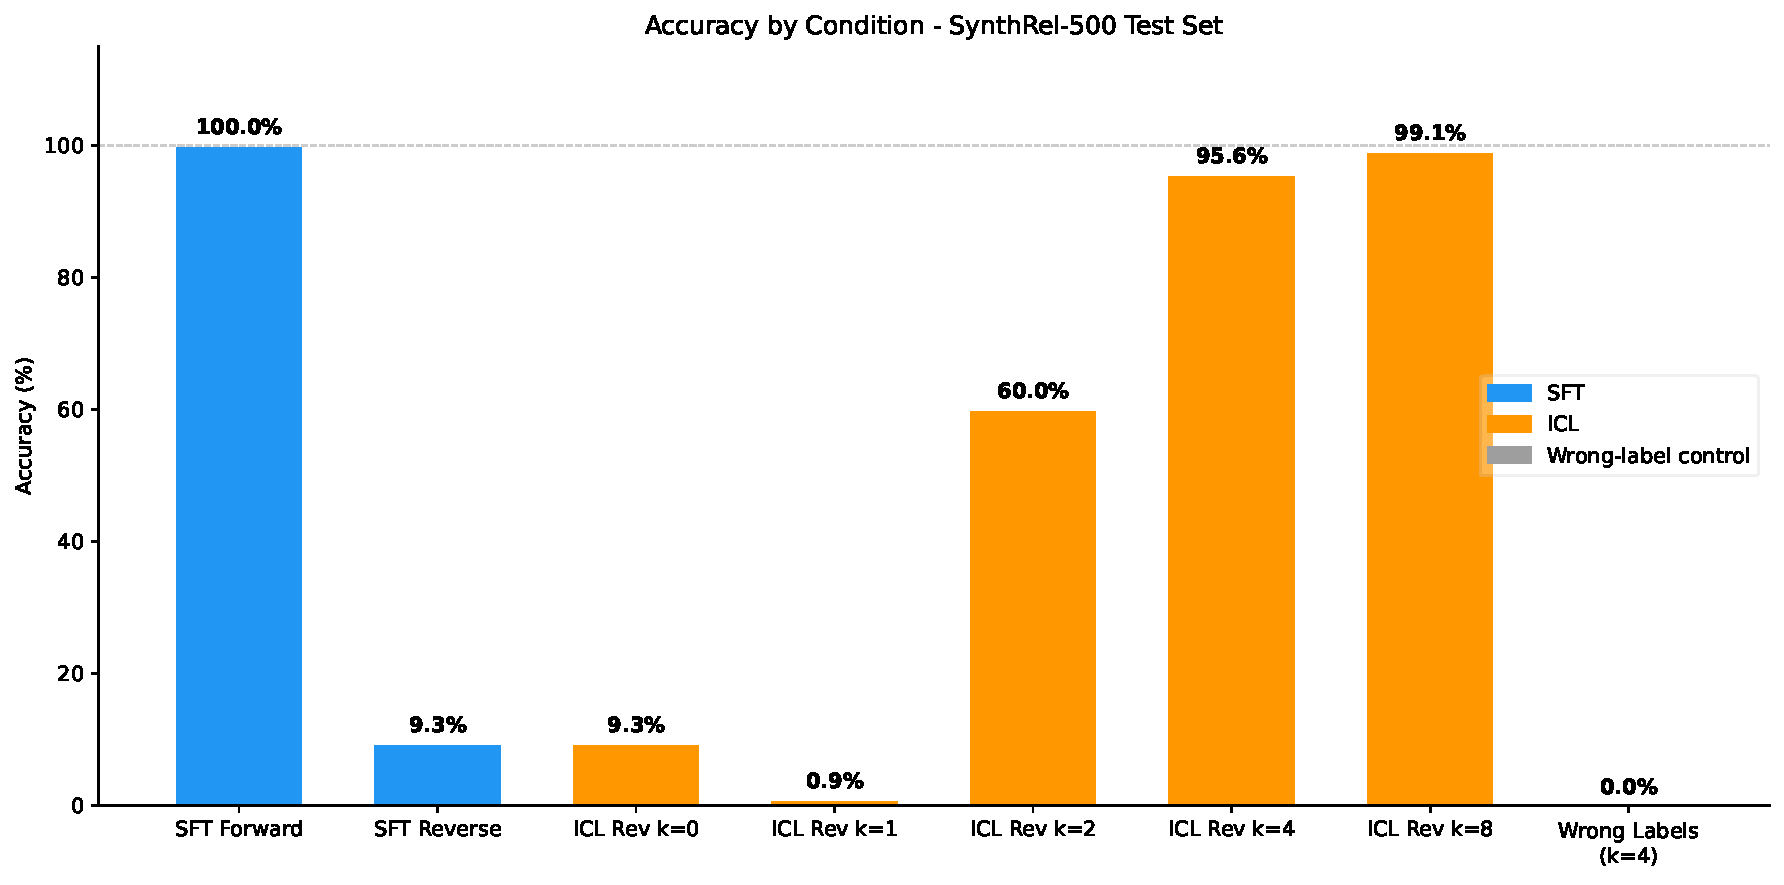
\includegraphics[width=\linewidth]{figures/gpt2_small/fig1.pdf}
  \caption{GPT-2 Small}
\end{subfigure}\hfill
\begin{subfigure}{0.48\textwidth}
  \centering
  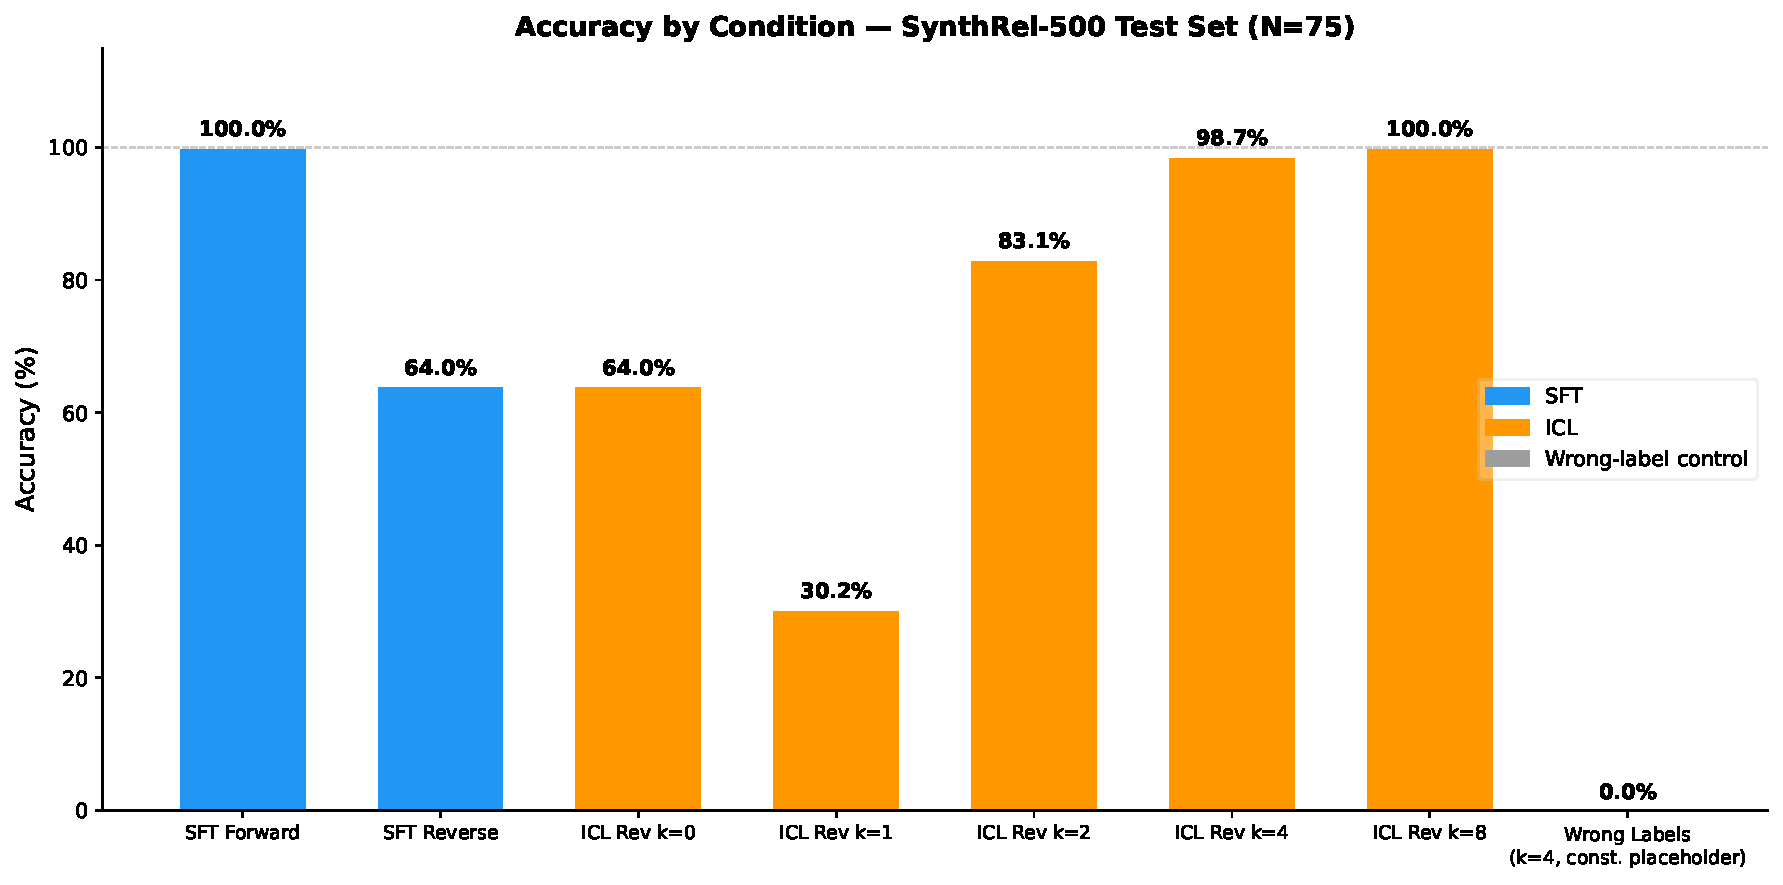
\includegraphics[width=\linewidth]{figures/gpt2_medium/fig1.pdf}
  \caption{GPT-2 Medium}
\end{subfigure}
\caption{Bar chart of primary accuracy conditions from Table~\ref{tab:main_results} for
Small and Medium. Blue = SFT conditions, orange = ICL conditions. The Large model
figure is in Appendix~\ref{app:largefigs}.}
\label{fig:fig1}
\end{figure}

\subsection{The $k=1$ Interference Effect Is Scale-Dependent}
\label{sec:kone}

Table~\ref{tab:main_results} reveals a scale-dependent, non-monotonic
relationship between demonstration count and ICL accuracy. In GPT-2 Small and
Medium, providing a single demonstration ($k=1$) causes accuracy to
\emph{collapse} below zero-shot performance: from 9.33\% to 0.89\% in Small,
and from 64.00\% to 30.22\% in Medium. In GPT-2 Large, however, $k=1$
\emph{improves} accuracy from 40.00\% to 75.11\%---a 35.11~pp gain. With two
or more demonstrations, accuracy recovers monotonically at all scales, reaching
near-ceiling at $k=4$.

\begin{figure}[H]
\centering
\begin{subfigure}{0.48\textwidth}
  \centering
  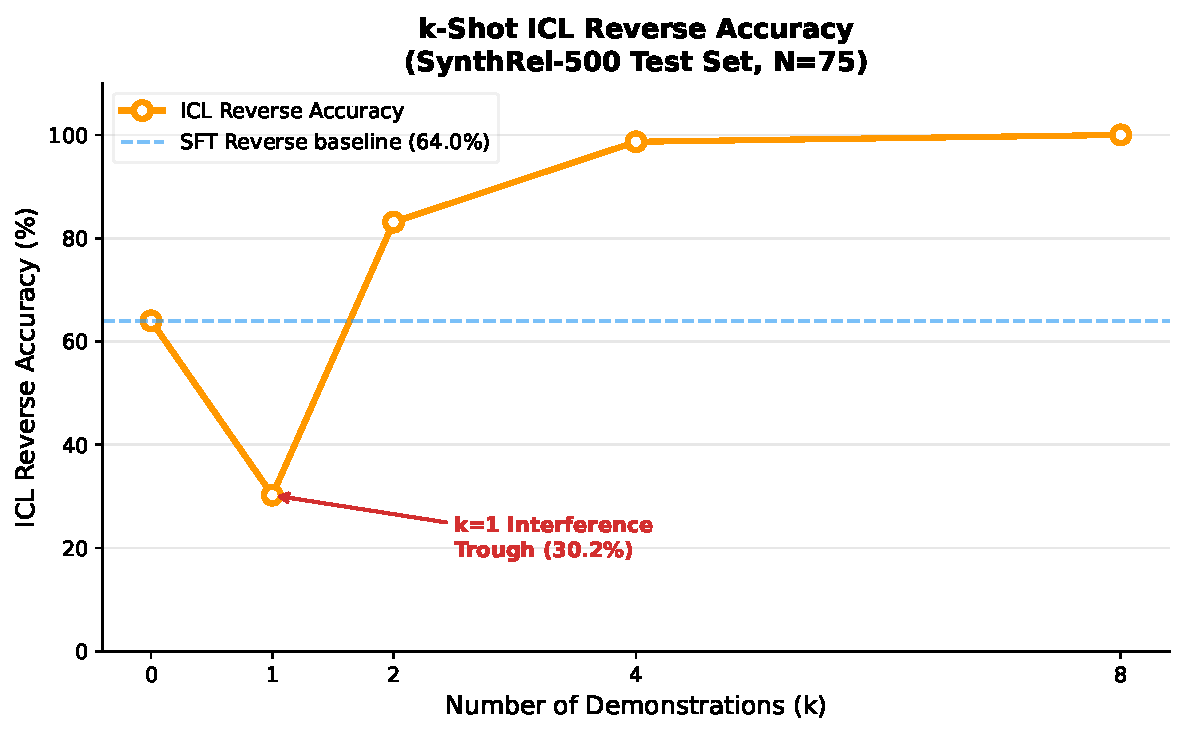
\includegraphics[width=\linewidth]{figures/gpt2_medium/fig2.pdf}
  \caption{GPT-2 Medium (interference at $k=1$)}
\end{subfigure}\hfill
\begin{subfigure}{0.48\textwidth}
  \centering
  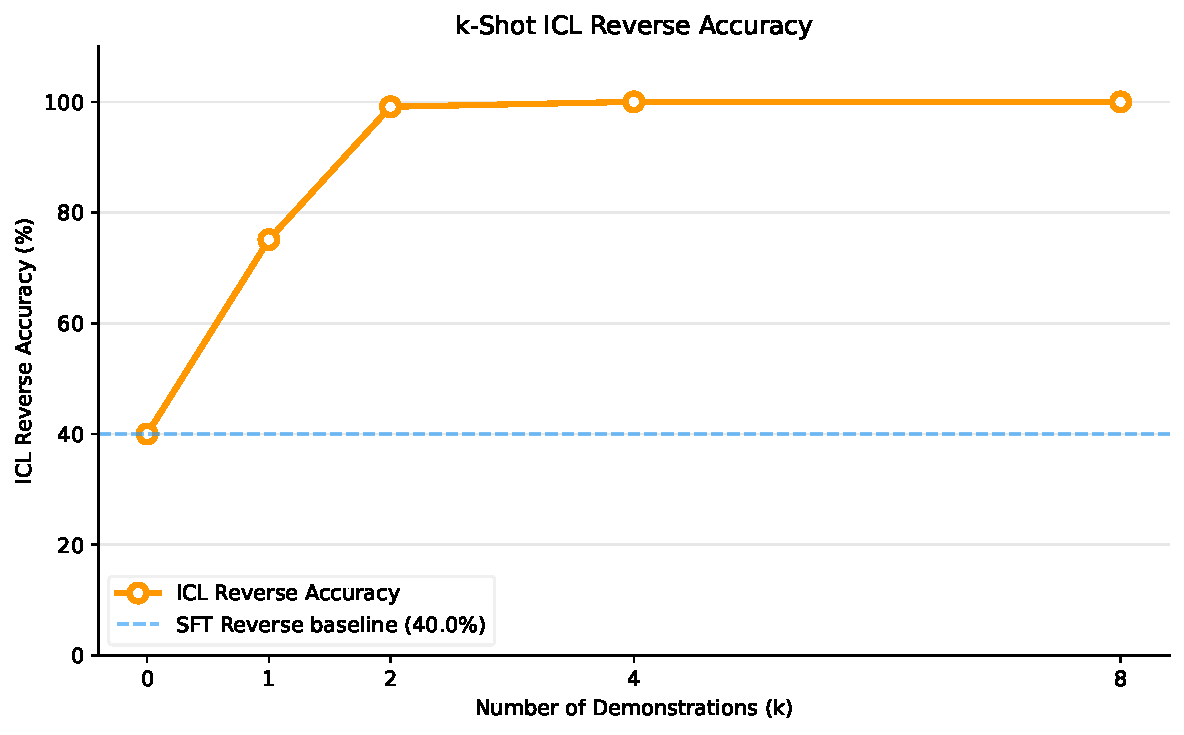
\includegraphics[width=\linewidth]{figures/gpt2_large/fig2.pdf}
  \caption{GPT-2 Large (improvement at $k=1$)}
\end{subfigure}
\caption{$k$-shot accuracy curves for Medium (left) and Large (right). The
non-monotonic trough at $k=1$ is present in Small and Medium but absent in Large,
demonstrating that the interference effect is scale-dependent.
See Appendix~\ref{app:smallfigs} for the Small model curve.}
\label{fig:fig2}
\end{figure}

We hypothesize a \emph{Mechanistic Interference Account} for the Small/Medium
behavior: induction circuits may implement prefix matching over \emph{repeated}
patterns. Under this account, with $k=0$ the model relies on parametric memory
from SFT, yielding moderate performance; with $k \geq 2$, a repeating structure
in context may activate induction heads that implement the reversal mapping; with
$k=1$, a single example disrupts parametric memory without establishing a
repeating pattern. The \emph{absence} of this effect in Large, where $k=1$
instead improves accuracy, is a positive finding that distinguishes the Large
model from Small and Medium. One interpretation is that a single demonstration
is sufficient to override parametric memory at larger scale---but we treat this
as a hypothesis, as the mechanism is not directly observed. The precise cause of
this scale dependence is an open question for future work.

\subsection{Robustness to Training Scale}
\label{sec:robustness}

To determine whether the Reversal Curse is a product of undertraining, we
evaluated SFT reverse accuracy across varying dataset sizes ($N = 35$ to
$N = 350$ examples) and training checkpoints for all three models.

\textbf{Dataset size.} Across all three models, increasing training data brings
forward accuracy to ceiling (100\% at $N \geq 140$ for Medium and Large, or at
$N = 350$ for Small) but does not rescue reverse accuracy:
\begin{itemize}
  \item \textit{Small:} $N=35$: forward 49.3\%, reverse 26.7\%; $N=350$: forward
  100\%, reverse 9.3\%. Reverse accuracy \emph{decreases} as forward accuracy
  improves.
  \item \textit{Medium:} $N=35$: forward 78.7\%, reverse 65.3\%; $N=350$:
  forward 100\%, reverse 64.0\%. Reverse accuracy is essentially flat (65.3\%
  to 64.0\%) while forward approaches ceiling.
  \item \textit{Large:} $N=35$: forward 97.3\%, reverse 60.0\%; $N=350$:
  forward 100\%, reverse 40.0\%. Similar to Small: as more data pushes forward
  to ceiling, reverse accuracy declines.
\end{itemize}

The consistent finding across scales is that adding training examples does not
help---and may slightly hurt---reverse accuracy, while fully saturating forward
accuracy. This confirms that the Reversal Curse is not a data-quantity problem.

\textbf{Training duration.} Checkpoint evaluations show that the accuracy gap
is established early and does not close with extended training: in Small and
Large, forward and reverse accuracy at checkpoint-100 are identical to the final
model; in Medium, the gap is slightly larger at checkpoint-100 but stabilizes
by checkpoint-200 with no further improvement in reverse accuracy.

% ============================================================
\section{Mechanistic Analysis: GPT-2 Medium}
\label{sec:mechanistic}
% ============================================================

The following sections report the complete mechanistic analysis for GPT-2
Medium, which provides the most data-rich setting (24 layers, $N=27$ eligible
items). Cross-scale mechanistic comparisons are presented in
Section~\ref{sec:scaling}.

\subsection{Activation Patching: Localizing the Reversal Bottleneck}
\label{sec:patching}

To identify \emph{where} in the network the Reversal Curse manifests, we
perform residual stream activation patching. To prevent positional embedding
collapse from sequence-length mismatch between SFT and ICL prompts, we pair
each ICL context with a token-length-matched corrupted prompt. For each test
example where SFT reverse is incorrect and ICL $k=4$ reverse is correct
($N=27$ items, i.e., all SFT reverse failures), we patch clean ICL activations
into the corrupted pass at each layer's \texttt{resid\_pre},
\texttt{attn\_out}, and \texttt{mlp\_out} positions and measure the resulting
logit improvement for the correct answer token.

\begin{table}[h]
\centering
\caption{Top causal locations by mean logit improvement when patching ICL
activations into the SFT reverse-failure case (GPT-2 Medium, $N=27$ items).}
\label{tab:patching}
\begin{tabular}{lcc}
\toprule
\textbf{Layer} & \textbf{Component} & \textbf{Mean Logit Improvement} \\
\midrule
16 & \texttt{resid\_pre} & $+3.97$ \\
17 & \texttt{resid\_pre} & $+3.95$ \\
18 & \texttt{resid\_pre} & $+3.93$ \\
15 & \texttt{attn\_out}  & $+1.24$ \\
\bottomrule
\end{tabular}
\end{table}

Logit improvement rises sharply beginning at layer 12 ($+1.95$), peaks at
layers 16--18 ($+3.97$, $+3.95$, $+3.93$), and remains elevated through layer
23. Early layers (0--5) show minimal improvement ($\sim 0.0$ to $0.13$),
showing that the reversal is not recoverable by early-layer interventions alone.
The peak and plateau from layer 16 onward implicates this window as the primary
causal site. This result is consistent with the hypothesis that forward-only
SFT encodes A$\to$B associations in early-to-mid MLP layers but does not install
the routing required at the residual stream entering layers 16--18 to support the
reverse direction.

\begin{figure}[H]
\centering
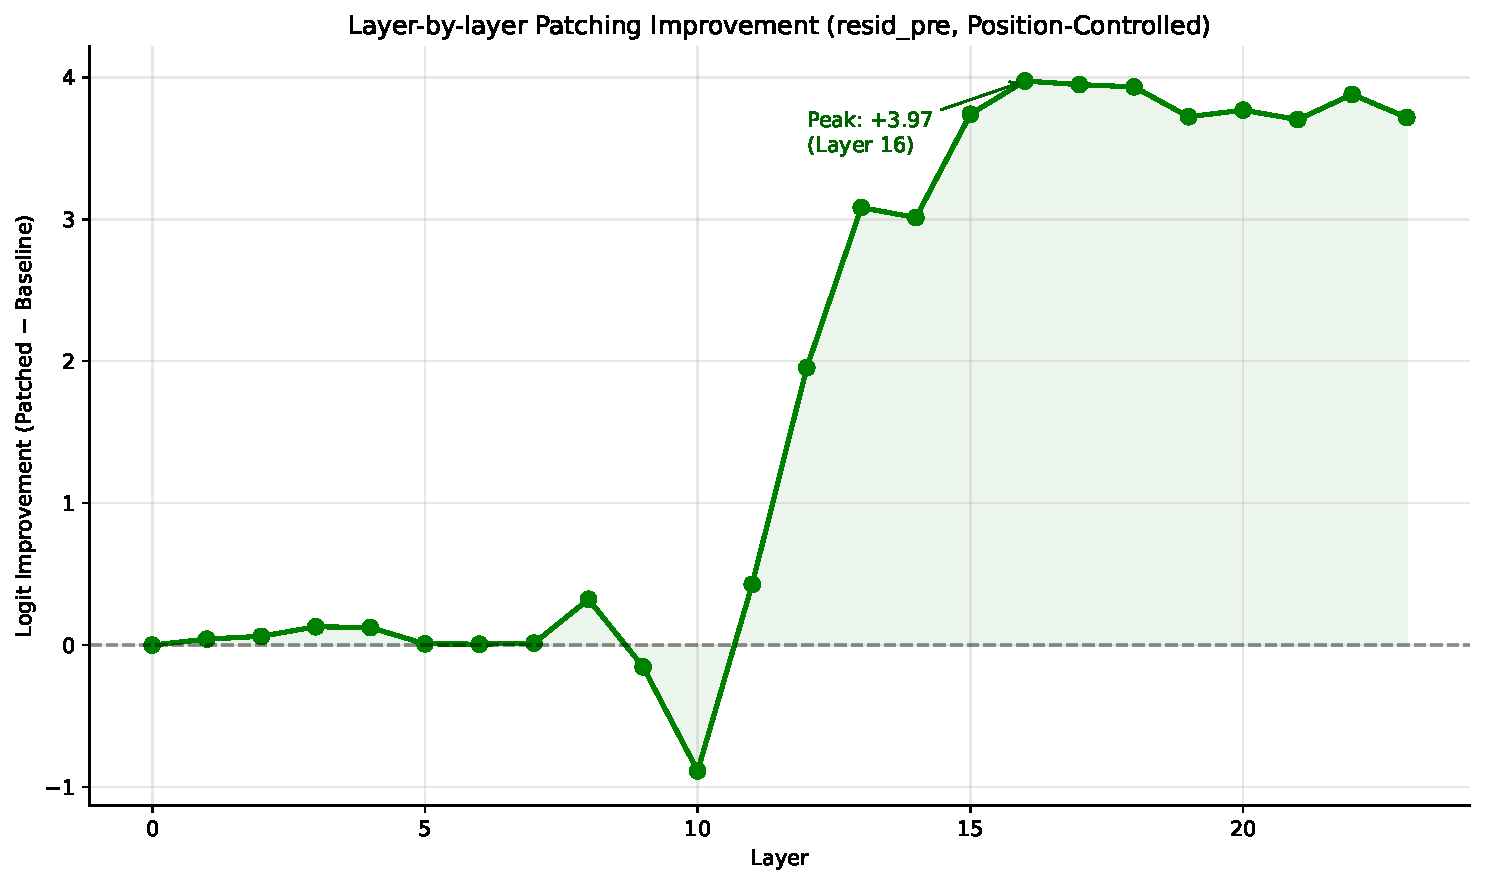
\includegraphics[width=0.8\textwidth]{figures/gpt2_medium/fig3.pdf}
\caption{Layer-by-layer patching improvement (resid\_pre) for GPT-2 Medium
across all 24 layers. For the full component breakdown including \texttt{attn\_out}
and \texttt{mlp\_out}, see Supplementary Figure~\ref{fig:figS1}.}
\label{fig:fig3}
\end{figure}

\subsection{Direct Logit Attribution: Dissociating ICL and SFT Circuits}
\label{sec:dla}

Direct Logit Attribution (DLA) decomposes the model's final logit for the
correct answer token into additive contributions from each attention head and
MLP sublayer, via the linearity of the residual stream. We compute DLA for the
final token position under three conditions: SFT forward (correct), SFT reverse
(incorrect), and ICL $k=4$ reverse (correct), over the $N=27$ eligible items.

The top-10 attention heads by mean signed ICL-reverse DLA (over all $N=75$ test
items) are shown in Table~\ref{tab:top_heads}. These heads are concentrated in
layers 14--23.

\begin{table}[h]
\centering
\caption{Top-10 attention heads by mean ICL-reverse DLA score over all $N=75$
test items (GPT-2 Medium), used to select ablation targets. The two rightmost
columns show mean DLA over the $N=27$ eligible subset (SFT reverse failures
where ICL succeeds) under ICL-reverse and SFT-forward conditions respectively,
for comparison. Heads are ranked by the $N=75$ ICL-reverse DLA column.}
\label{tab:top_heads}
\begin{tabular}{cccccc}
\toprule
\textbf{Rank} & \textbf{Layer} & \textbf{Head} & \textbf{ICL Rev DLA ($N=75$)} & \textbf{ICL Rev ($N=27$)} & \textbf{SFT Fwd ($N=27$)} \\
\midrule
1  & 15 & 14 & 37.09 & 34.79 & 16.86 \\
2  & 20 &  7 & 32.64 & 22.12 & 27.46 \\
3  & 18 & 12 & 25.64 & 28.70 & 33.68 \\
4  & 18 &  5 & 21.06 & 11.90 & 16.17 \\
5  & 19 & 15 & 17.86 & 10.47 & 10.96 \\
6  & 14 & 14 & 17.40 & 15.25 &  3.22 \\
7  & 16 & 15 & 16.49 & 14.03 & 15.99 \\
8  & 20 & 12 & 15.09 &  8.25 & 15.76 \\
9  & 20 &  4 & 15.07 & 13.80 & 14.30 \\
10 & 23 &  6 & 14.28 & 18.17 & 13.88 \\
\bottomrule
\end{tabular}
\end{table}

Notably, the top-10 heads ranked by absolute ICL DLA do not themselves show
strong SFT/ICL dissociation (mean per-head DLA 17.75 vs.\ 16.83 over the
$N=27$ subset); these heads are high-magnitude contributors in both conditions.
The significant dissociation emerges at the layer level, as we show below.

Statistical analysis via Wilcoxon signed-rank tests on per-example DLA scores
(over the $N=27$ eligible subset), with Benjamini-Hochberg correction across
layers, is consistent with a systematic dissociation in both attention and MLP
routing.

For \textbf{attention routing}, ICL significantly out-recruits SFT in eight
early-to-mid layers (6, 7, 9--11, 13--15), all with negative rank-biserial $r$
(ICL $>$ SFT), consistent with a broadly distributed attention contribution to
ICL reversal. Layer 22 shows the opposite (SFT $>$ ICL, $r = +0.841$),
consistent with a late-layer parametric write that ICL bypasses. The full
breakdown is in Table~\ref{tab:dla_sig}. Layer-wise totals (summed across all
16 heads) in Table~\ref{tab:layer_dla_raw} show the scale of this shift: ICL
DLA is higher at layers 6--15 while SFT DLA is higher at layer 22.

\begin{table}[H]
\centering
\caption{Mean Layer-Wise Attention DLA (summed across all 16 heads per layer)
for $N=27$ eligible items, GPT-2 Medium.}
\label{tab:layer_dla_raw}
\begin{tabular}{cccccc}
\toprule
\textbf{Layer} & \textbf{SFT Mean} & \textbf{ICL Mean} & \textbf{Layer} & \textbf{SFT Mean} & \textbf{ICL Mean} \\
\midrule
 0 &   1.47 &   2.17 & 12 &  18.88 &  13.88 \\
 1 &   0.50 &  -2.67 & 13 &  22.03 &  33.48 \\
 2 &   3.76 &   5.49 & 14 &  17.70 &  51.02 \\
 3 &   0.96 &   1.39 & 15 &  63.17 &  98.88 \\
 4 &   0.34 &  -0.84 & 16 &  45.38 &  47.87 \\
 5 &   0.91 &   0.89 & 17 &  54.20 &  59.72 \\
 6 &   6.55 &  11.08 & 18 & 127.05 & 117.36 \\
 7 &   1.67 &   5.67 & 19 &  94.49 &  70.14 \\
 8 &   1.69 &  -0.10 & 20 & 165.61 & 151.20 \\
 9 &   4.57 &  17.12 & 21 & 137.17 & 101.99 \\
10 &   1.67 &   9.34 & 22 &  76.12 &  28.65 \\
11 &   3.38 &  10.77 & 23 &  96.13 &  90.77 \\
\bottomrule
\end{tabular}
\end{table}

\begin{table}[H]
\centering
\caption{Significant differences in Attention DLA (ICL Reverse vs.\ SFT
Forward, $N=27$, GPT-2 Medium). Negative rank-biserial $r$ indicates ICL
$>$ SFT; positive $r$ indicates SFT $>$ ICL. Layers 6--15 form a distributed
early-to-mid population recruited more strongly by ICL; layer 22 reflects a
late-layer parametric trace more strongly recruited by SFT.}
\label{tab:dla_sig}
\begin{tabular}{ccccc}
\toprule
\textbf{Layer} & \textbf{Wilcoxon Stat} & \textbf{Raw $p$-value} & \textbf{BH-corrected $p$} & \textbf{Rank-Biserial $r$} \\
\midrule
 6 &  90.0 & $0.016$            & $0.043$             & $-0.524$ \\
 7 &  68.0 & $0.003$            & $0.008$             & $-0.640$ \\
 9 &  14.0 & $1.64\times10^{-6}$ & $1.31\times10^{-5}$ & $-0.926$ \\
10 &  63.0 & $0.002$            & $0.006$             & $-0.667$ \\
11 &  54.0 & $0.001$            & $0.003$             & $-0.714$ \\
13 &  19.0 & $4.57\times10^{-6}$ & $2.74\times10^{-5}$ & $-0.899$ \\
14 &   0.0 & $1.49\times10^{-8}$ & $3.58\times10^{-7}$ & $-1.000$ \\
15 &   4.0 & $1.04\times10^{-7}$ & $1.25\times10^{-6}$ & $-0.979$ \\
22 &  30.0 & $<0.001$           & $0.015$             & $+0.841$ \\
\bottomrule
\end{tabular}
\end{table}

For \textbf{MLP routing}, the dissociation is complementary: early-to-mid MLP
sublayers (layers 10, 12, 13) contribute more to SFT forward predictions than
to ICL reverse predictions (SFT $>$ ICL), consistent with these layers storing
learned forward A$\to$B associations. Mid-to-late MLP sublayers (layers 15,
17--20) show the opposite: ICL significantly out-recruits SFT ($r \approx
-0.53$ to $-0.70$), indicating that ICL actively recruits late MLP layers as a
processing substrate for the reversed relationship. Details are in
Table~\ref{tab:dla_sig_mlp}.

\begin{table}[H]
\centering
\caption{Significant differences in MLP DLA (ICL Reverse vs.\ SFT Forward,
$N=27$, GPT-2 Medium). Negative rank-biserial $r$ indicates ICL $>$ SFT.}
\label{tab:dla_sig_mlp}
\begin{tabular}{ccccc}
\toprule
\textbf{Layer} & \textbf{Wilcoxon Stat} & \textbf{Raw $p$-value} & \textbf{BH-corrected $p$} & \textbf{Rank-Biserial $r$} \\
\midrule
10 & 48.0 & $0.0003$ & $0.008$ & $+0.746$ \\
12 & 70.0 & $0.003$  & $0.016$ & $+0.630$ \\
13 & 81.0 & $0.008$  & $0.028$ & $+0.571$ \\
15 & 67.0 & $0.002$  & $0.015$ & $-0.646$ \\
17 & 62.0 & $0.002$  & $0.012$ & $-0.672$ \\
18 & 76.0 & $0.005$  & $0.022$ & $-0.598$ \\
19 & 89.0 & $0.015$  & $0.045$ & $-0.529$ \\
20 & 57.0 & $0.001$  & $0.011$ & $-0.698$ \\
\bottomrule
\end{tabular}
\end{table}

\begin{figure}[H]
\centering
\begin{subfigure}{\textwidth}
  \centering
  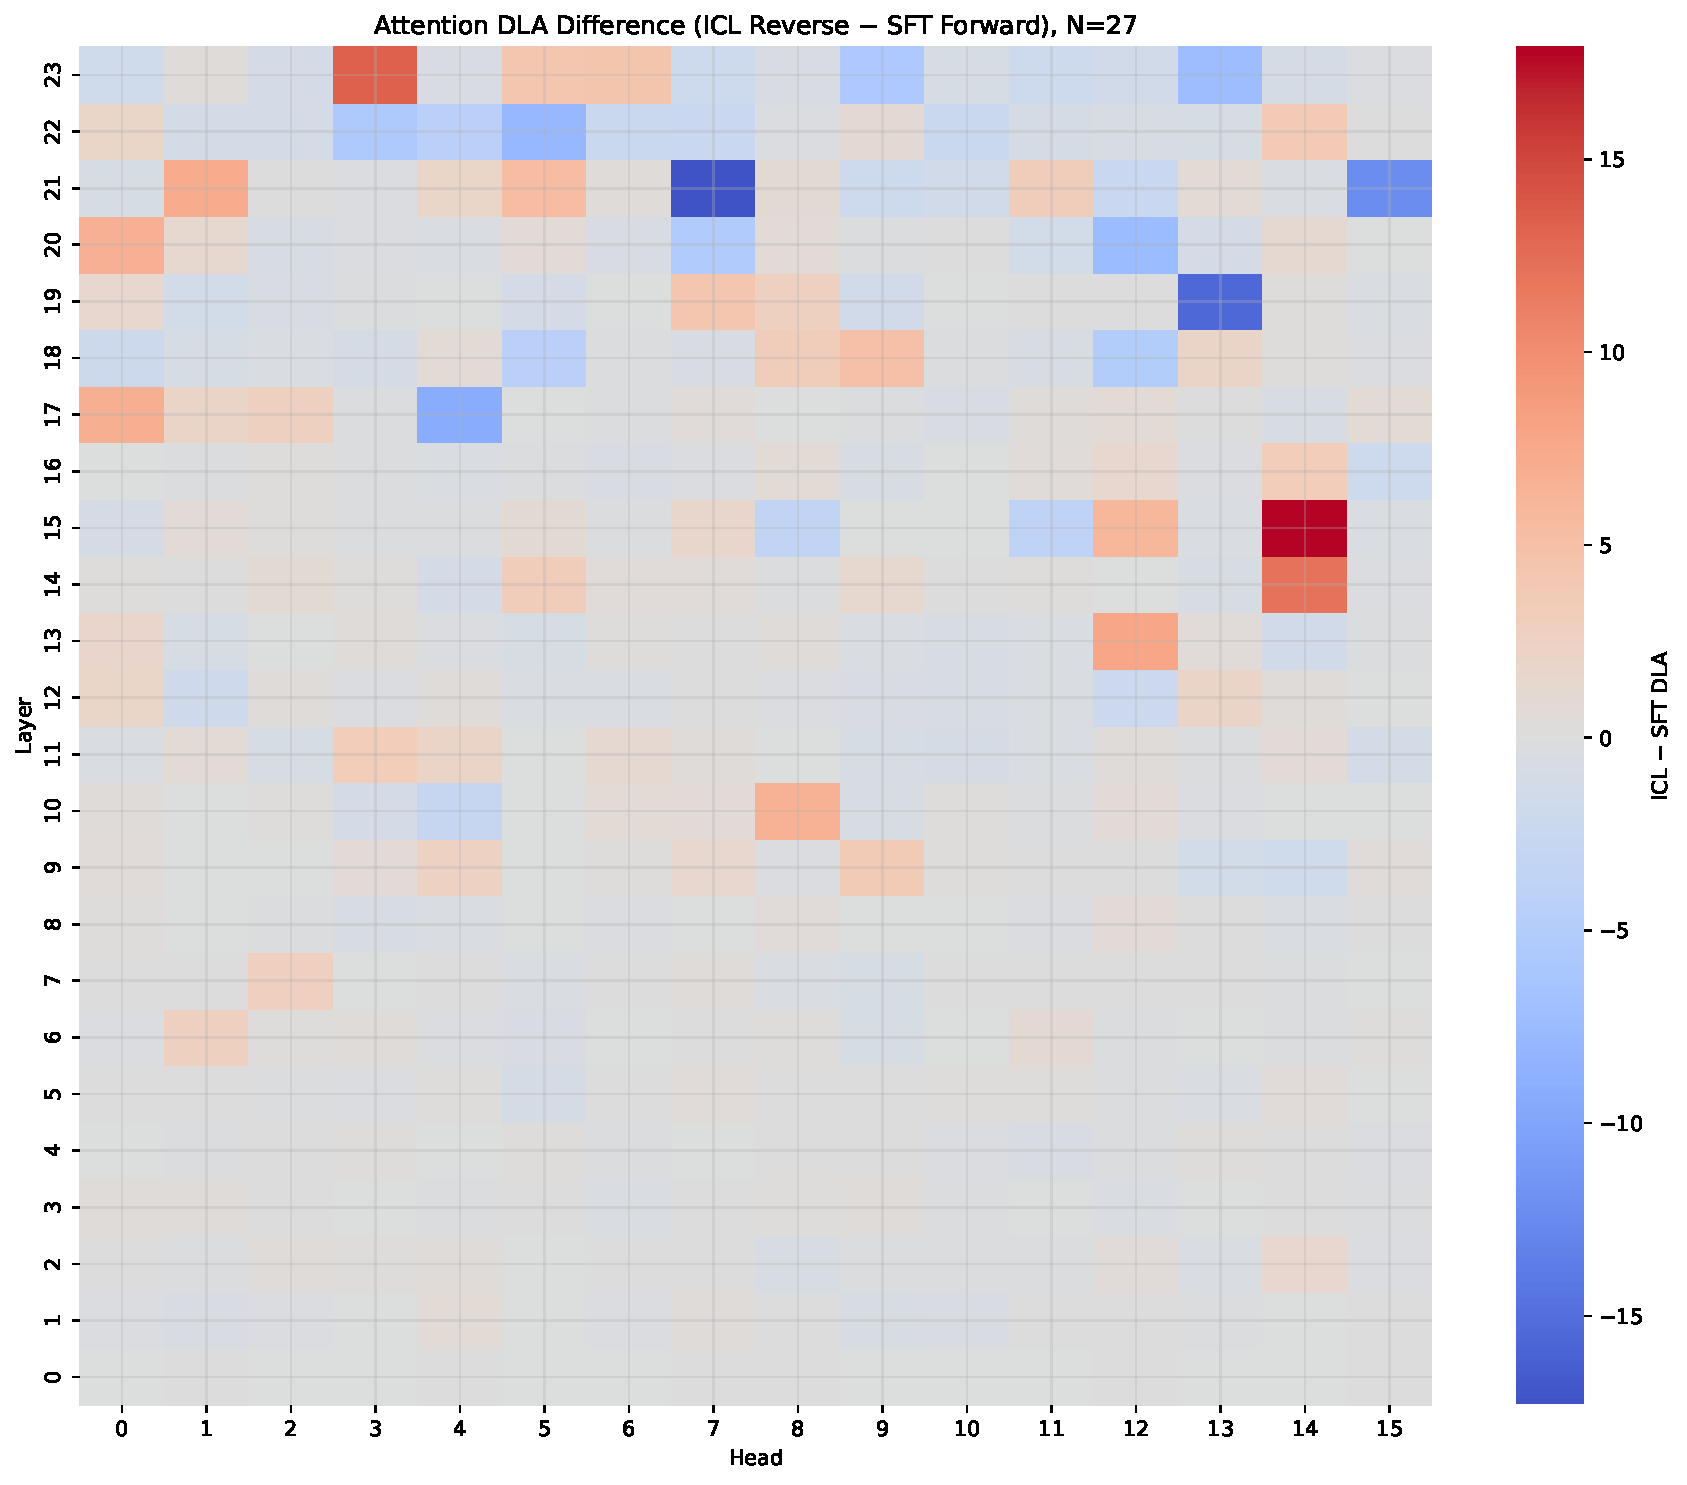
\includegraphics[width=0.8\linewidth]{figures/gpt2_medium/fig4a.pdf}
  \caption{DLA heatmap (attention heads) for ICL reverse vs.\ SFT forward,
  GPT-2 Medium.}
\end{subfigure}\\
\begin{subfigure}{\textwidth}
  \centering
  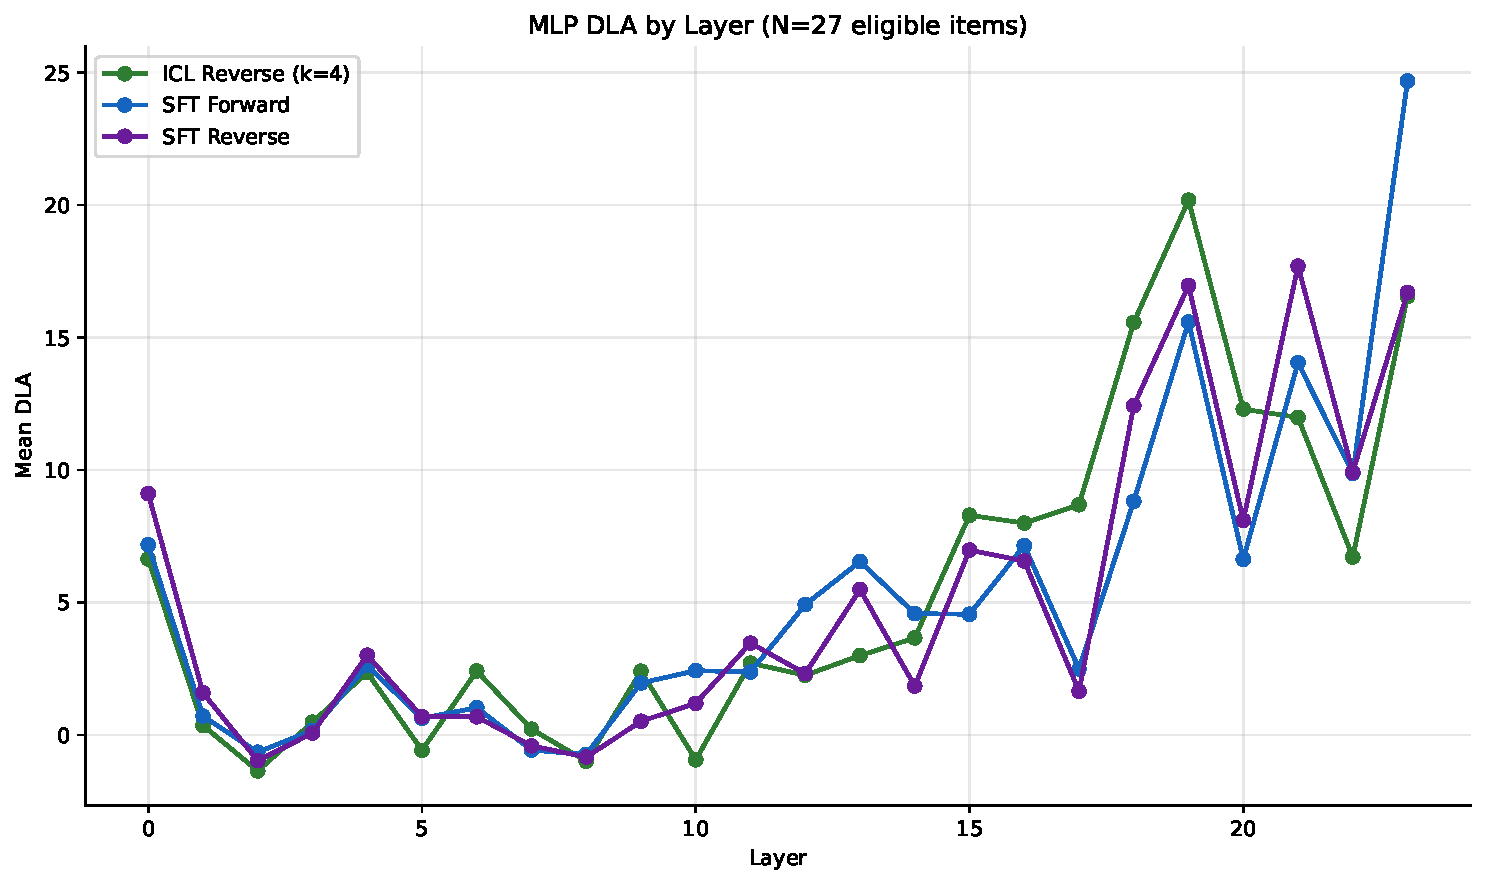
\includegraphics[width=0.8\linewidth]{figures/gpt2_medium/fig4b.pdf}
  \caption{MLP DLA by layer for SFT forward, SFT reverse, and ICL reverse
  conditions, GPT-2 Medium.}
\end{subfigure}
\caption{DLA Heatmaps for Attention (top) and MLP (bottom) components,
GPT-2 Medium.}
\label{fig:fig4}
\end{figure}

\subsection{Structural Ablation Studies}
\label{sec:ablation}

We conduct two large-scale structural ablations to test the causal role of the
circuits identified in the DLA analysis.

\paragraph{Attention Head Ablation.}
We simultaneously zero-ablate (set \texttt{hook\_z} output to zero) the 10
attention heads with the highest signed mean ICL-reverse DLA over all $N=75$
test items, using relation-matched $k=4$ demonstrations. These are the heads
listed in Table~\ref{tab:top_heads}. This targets the highest-scoring
final-write heads, which are not the same set as the dissociation-specific
layers identified in Section~\ref{sec:dla}. We evaluate this ablation on the
primary model and on three independently trained replicate models (seeds 101,
202, 303).

\begin{table}[H]
\centering
\caption{Attention head ablation results for GPT-2 Medium across the primary
model and three replicates. Head overlap is reported as the signed-DLA-over-$N=75$
diagnostic against the primary model's top-10 list.}
\label{tab:ablation_results}
\begin{tabular}{lcccc}
\toprule
\textbf{Model} & \textbf{Unablated ICL Rev} & \textbf{Ablated ICL Rev} & \textbf{$\Delta$} & \textbf{Head Overlap} \\
\midrule
Primary model & 98.22\% & 78.22\% & $-20.00$~pp & --- \\
Seed 101      & 98.22\% & 78.67\% & $-19.55$~pp & 10/10 \\
Seed 202      & 98.22\% & 86.67\% & $-11.55$~pp & 10/10 \\
Seed 303      & 99.56\% & 89.33\% & $-10.23$~pp & 10/10 \\
\bottomrule
\end{tabular}
\end{table}

SFT forward accuracy under ablation was measured for the primary model only
(single-token argmax: 100.00\%); it was not re-evaluated under ablation for the
three replicates. The effect is consistent in direction across all four runs but
varies in magnitude by roughly a factor of two (10.23--20.00~pp), indicating
that these heads are involved in ICL reversal while the network retains
meaningful redundancy. The ablation does not isolate a singular necessary
bottleneck.

Independently of ablation magnitude, the identity of the top-10 heads under the
signed-DLA-over-$N=75$ diagnostic is stable across seeds: all three replicate
models share all 10 heads with the primary model's list. ICL reversal appears
to consistently recruit the same high-DLA attention population across independent
training runs, even as the causal dependence on those heads varies.

\paragraph{Single-Layer MLP Ablation Sweep.}
We sequentially zero-ablate the \texttt{mlp\_out} of individual layers from
layer 6 through layer 18. Results:

\begin{itemize}
  \item \textit{SFT Forward:} Accuracy drops by up to 3.7~pp (at layer 13),
  evaluated via single-token argmax.
  \item \textit{ICL Reverse:} Remains at 100.0\% across every single ablated
  layer.
\end{itemize}

Individual mid-to-late MLP layers appear involved in SFT forward memorization
but are individually dispensable for ICL reverse decoding. This is inconsistent
with the hypothesis that ICL relies on the same specific parametric traces as
SFT.

\paragraph{Combined MLP Ablation.}
Combined zero-ablation of all 13 of these MLP layers simultaneously causes ICL
reverse accuracy to collapse to \textbf{0.00\%} and SFT forward accuracy to
degrade to \textbf{45.33\%}. Both modalities appear to rely on the MLP ensemble
as a shared computational substrate; ICL does not appear to operate without it,
even though individual MLP layers are individually dispensable.

\begin{figure}[H]
\centering
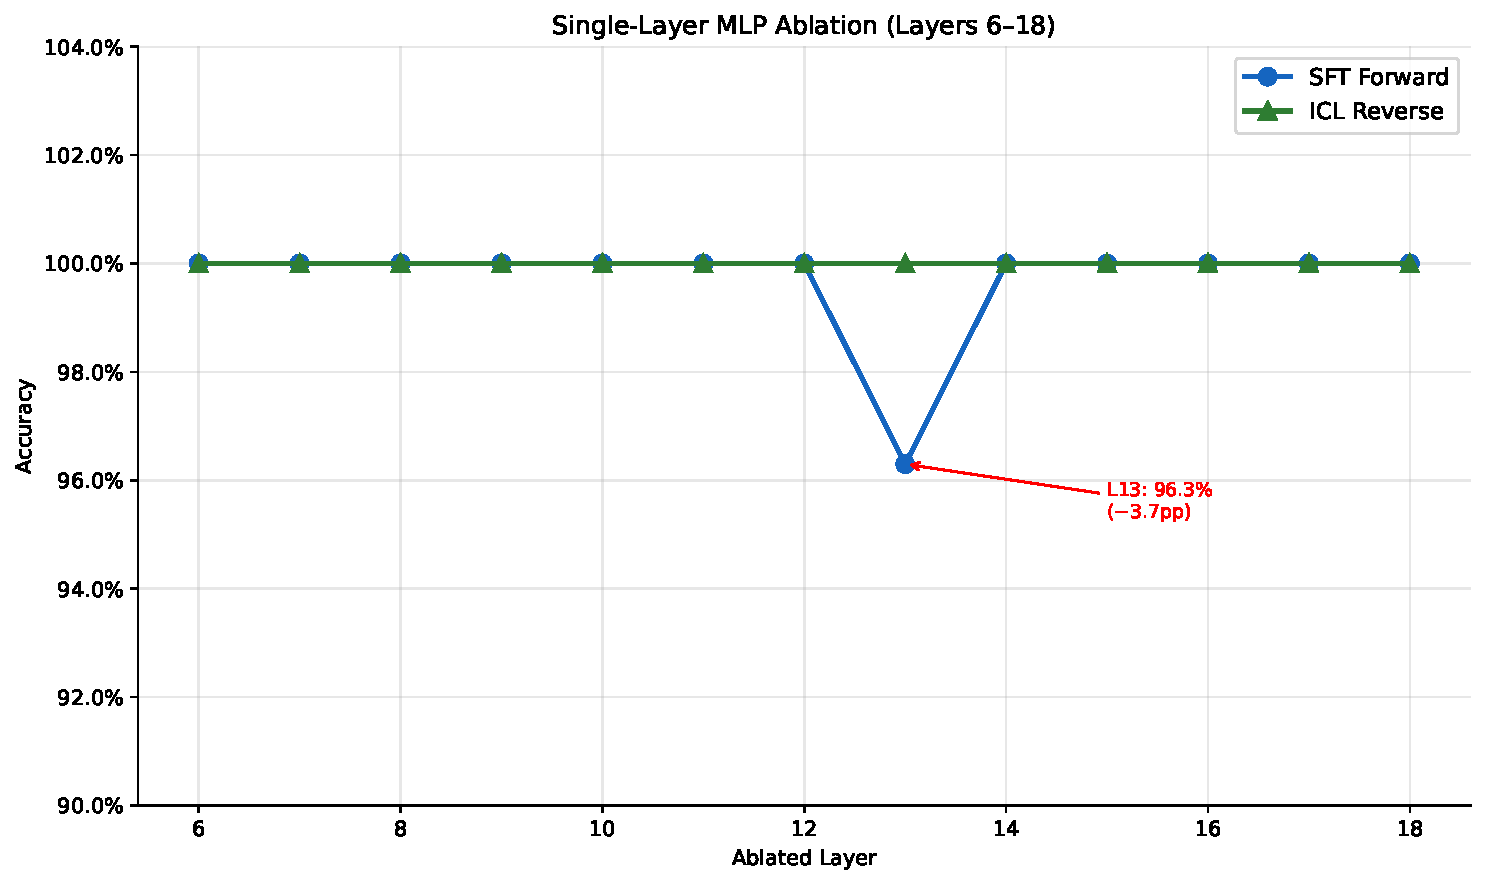
\includegraphics[width=0.8\textwidth]{figures/gpt2_medium/fig5.pdf}
\caption{Single-layer MLP ablation sweep across layers 6--18, GPT-2 Medium.
SFT forward accuracy drops at layer 13 while ICL reverse accuracy remains at
100\%. Note that this ablation uses single-token argmax rather than the
full-sequence exact-match metric of Table~\ref{tab:main_results}, yielding a
higher SFT forward baseline.}
\label{fig:fig5}
\end{figure}

% ============================================================
\section{Cross-Scale Analysis}
\label{sec:scaling}
% ============================================================

Having characterized the mechanism in detail for GPT-2 Medium, we now compare
key mechanistic properties across all three model scales to identify which
aspects of the mechanism are scale-invariant and which change with model size.

\subsection{Activation Patching: Layer Position Scales with Depth}

Table~\ref{tab:patching_comparison} summarizes the patching bottleneck location
across all three models.

\begin{table}[H]
\centering
\caption{Activation patching bottleneck across model scales. Peak layer reports
the layer with maximum \texttt{resid\_pre} logit improvement.}
\label{tab:patching_comparison}
\begin{tabular}{lcccc}
\toprule
\textbf{Model} & \textbf{Total Layers} & \textbf{Peak Layer} & \textbf{Peak Logit Improvement} & \textbf{Relative Position} \\
\midrule
GPT-2 Small  & 12 & 10--11 & $+6.70$ & 83--92\% \\
GPT-2 Medium & 24 & 16--18 & $+3.97$ & 67--75\% \\
GPT-2 Large  & 36 & 22--25 & $+6.83$ & 61--69\% \\
\bottomrule
\end{tabular}
\end{table}

The causal intervention effect consistently peaks in the upper portion of the
network at all scales, though it shifts slightly earlier in relative terms as the
model grows deeper. Early layers (bottom 50\%) show minimal patching improvement
at all scales, showing that the reversal is not recoverable by early-layer
interventions alone. The consistency of this relative position across scales is
consistent with, though does not prove, the hypothesis that this layer range
reflects a transition from stored factual representations to final prediction
routing---a computation that may require sufficient representational depth
regardless of model scale.

\subsection{Attention Head Ablation: Redundancy Increases with Scale}

Table~\ref{tab:ablation_cross_scale} reports the primary model attention head
ablation results across all three scales.

\begin{table}[H]
\centering
\caption{Attention head ablation results for the primary model at each scale.
Unablated accuracy is from Table~\ref{tab:main_results}; ablated accuracy
is from the ablation script (which uses single-token argmax, yielding slightly
different baselines for Small and Medium).}
\label{tab:ablation_cross_scale}
\begin{tabular}{lcccc}
\toprule
\textbf{Model} & \textbf{Unablated ICL Rev} & \textbf{Ablated ICL Rev} & \textbf{$\Delta$ ICL} & \textbf{$\Delta$ SFT Fwd} \\
\midrule
GPT-2 Small  & 95.56\% & 49.33\% & $-46.22$~pp & $-25.33$~pp \\
GPT-2 Medium & 98.22\% & 78.22\% & $-20.00$~pp &  0.00~pp \\
GPT-2 Large  & 100.00\% & 100.00\% & \phantom{0}$0.00$~pp &  $-1.33$~pp \\
\bottomrule
\end{tabular}
\end{table}

The ablation effect decreases sharply with model scale: $-46$~pp in Small,
$-20$~pp in Medium, and effectively $0$~pp in Large. The zero effect in Large
is an informative positive result: the top-10 ICL attention heads can be
entirely removed without measurable performance loss, suggesting that ICL
routing becomes substantially more redundant as model size increases. In GPT-2
Large, other heads or circuit components appear to fully compensate for the
ablated population.

Head identity stability under the signed-DLA-over-$N=75$ diagnostic is
generally high, though it decreases modestly with scale: 10/10 overlap in all
three Medium replicate seeds, 9/10 in all three Small replicate seeds, and
8--9/10 in Large replicate seeds. Head identity therefore appears to reflect a
consistently learned circuit feature across scales, even as causal dependence
on that circuit (measured by ablation) diminishes substantially.

\begin{table}[H]
\centering
\caption{Head stability and ablation results across all three scales and all
replicate seeds. Unablated ICL accuracy is from the replicate seed evaluation
(slightly different from Table~\ref{tab:main_results} due to evaluation mode).}
\label{tab:stability_cross_scale}
\begin{tabular}{llccc}
\toprule
\textbf{Model} & \textbf{Seed} & \textbf{Head Overlap} & \textbf{Ablated ICL Rev} & \textbf{Ablated SFT Fwd} \\
\midrule
\multirow{3}{*}{Small}  & 101 & 9/10 & 43.56\% & 72.00\% \\
                        & 202 & 9/10 & 36.00\% & 40.00\% \\
                        & 303 & 9/10 & 52.00\% & 82.67\% \\
\midrule
\multirow{3}{*}{Medium} & 101 & 10/10 & 78.67\% & --- \\
                        & 202 & 10/10 & 86.67\% & --- \\
                        & 303 & 10/10 & 89.33\% & --- \\
\midrule
\multirow{3}{*}{Large}  & 101 &  9/10 & 37.33\% & 82.67\% \\
                        & 202 &  8/10 & 100.00\% & 100.00\% \\
                        & 303 &  9/10 & 93.33\% & 100.00\% \\
\bottomrule
\end{tabular}
\end{table}

The Large model seed results (Table~\ref{tab:stability_cross_scale}) reveal
substantial instability: seed 101 achieves only 48.44\% unablated ICL k=4
accuracy (vs.\ 100\% for the primary and other seeds) and 61.33\% SFT forward
accuracy, indicating incomplete convergence during training. This training
instability is separate from the ablation-magnitude variance noted above and
suggests that the Large model training recipe (350 examples, 5 epochs) is
approaching its reliability limits at this scale.

\subsection{MLP Substrate: Universal Dependency Across Scales}

Combined MLP ablation (Table~\ref{tab:mlp_combined}) produces dramatic effects
at all scales, confirming the universal dependency on the MLP ensemble.

\begin{table}[H]
\centering
\caption{Combined MLP ablation results across all three scales. Each model
ablates its own scale-specific MLP layer range; Small ablates 6 layers (6--11),
Medium and Large ablate 13 layers (6--18).}
\label{tab:mlp_combined}
\begin{tabular}{lccccc}
\toprule
\textbf{Model} & \textbf{Ablated Layers} & \textbf{ICL Rev (Pre)} & \textbf{ICL Rev (Post)} & \textbf{SFT Fwd (Pre)} & \textbf{SFT Fwd (Post)} \\
\midrule
GPT-2 Small  & 6--11 & 95.56\% & 92.00\% & 100.00\% & 46.67\% \\
GPT-2 Medium & 6--18 & 98.67\% &  0.00\% & 100.00\% & 45.33\% \\
GPT-2 Large  & 6--18 & 100.00\% & 0.00\% & 100.00\% &  0.00\% \\
\bottomrule
\end{tabular}
\end{table}

ICL collapses completely (0\%) under combined MLP ablation in Medium and Large.
Small shows a smaller but still substantial drop (to 92\%), likely because only
6 of 12 layers are ablated rather than 13. SFT forward accuracy also degrades
severely, indicating that the MLP ensemble serves as a shared processing
substrate for both modalities. In Large, both ICL and SFT reach 0\% after
combined ablation, suggesting that the MLPs in layers 6--18 of the 36-layer
model are even more critical to overall function than in Medium.

\subsection{Top Attention Heads: Layer Position Scales with Depth}

The top-10 ICL-reverse DLA heads shift in absolute layer position with scale,
while remaining in the middle-to-upper portion of the network:

\begin{itemize}
  \item \textit{Small:} Concentrated in layers 6--11 (of 12), approximately the
  50th--92nd percentile; top head at Layer 10, Head 10 (DLA: 43.43).
  \item \textit{Medium:} Concentrated in layers 14--23 (of 24), approximately
  the 58th--96th percentile; top head at Layer 15, Head 14 (DLA: 37.09).
  \item \textit{Large:} Concentrated in layers 22--30 (of 36), approximately
  the 61st--83rd percentile; top head at Layer 23, Head 7 (DLA: 9.94).
\end{itemize}

The absolute DLA magnitudes decrease substantially across scales (Small: 43.43;
Medium: 37.09; Large: 9.94), which together with the zero ablation effect in
Large is consistent with the DLA signal being distributed across more heads in
larger models---each contributing less individually, but collectively maintaining
function even when the top-10 are removed.

\subsection{Induction-Head Properties Decrease with Scale}

Induction-score verification (using random repeated-token sequences with a
$>0.40$ threshold) shows a decreasing fraction of the top-10 DLA heads passing
the induction criterion with scale: 5/10 in Small, 5/10 in Medium, and 2/10 in
Large (see Appendix~\ref{app:induction} for full tables). In Large, only heads
at Layer 27, Head 17 (score 0.732) and Layer 26, Head 3 (score 0.445) pass the
threshold, while the remaining eight high-DLA heads score below 0.38. This
suggests that as models scale, the high-DLA ICL-relevant heads become less
induction-like in character, potentially reflecting different algorithmic
strategies for in-context relational retrieval.

% ============================================================
\section{Discussion}
\label{sec:discussion}
% ============================================================

\subsection{A Proposed Mechanistic Account}

Our results are consistent with the following account of the Reversal Curse
and its ICL circumvention. We note that this account is a hypothesis grounded
in the observed evidence, not a demonstrated mechanism.

\textbf{Forward-only SFT appears to encode factual associations asymmetrically.}
Consistent with Geva et~al.~\cite{geva2021transformer} and
Meng et~al.~\cite{meng2022locating}, forward-only SFT appears to install
key-value associations in early-to-mid MLP layers (e.g., layers 10--13 in
Medium), with A as the retrieval key and B as the retrieved value. No
corresponding B$\to$A association appears to be installed, as the gradient
signal never requires the model to predict A from B. This asymmetry is
observed at all three scales.

\textbf{The causal intervention evidence implicates the upper portion of the network.}
Activation patching implicates the upper one-third of the network as the
critical failure point at all three scales. The causal intervention effect peaks
consistently in the late-mid to late layers regardless of model depth, consistent
with the hypothesis that this layer range is where the routing from B toward A
must be established.

\textbf{ICL appears to engage distributed attention routing rather than a sparse dedicated circuit.}
DLA in Medium shows that ICL is associated with higher residual stream
contributions from a broad population of early-to-mid layer attention heads
relative to SFT. The consistent degradation upon ablation of these heads in
Small ($-46$~pp) and Medium ($-20$~pp), replicated across independent training
runs, is consistent with a causal role for this population in ICL reversal.
The \emph{absence} of any ablation effect in Large is an equally informative
finding: it suggests that ICL routing becomes substantially more redundant at
larger scale, such that no single subset of 10 attention heads is necessary.

\textbf{ICL does not appear to operate independently of MLP computation.}
Combined MLP ablation collapses ICL at Medium and Large. ICL does not appear
to operate without the MLP ensemble, even though individual MLP layers are
individually dispensable. One plausible interpretation is that MLP layers
compute relational entity representations that attention heads use to perform
context-driven pattern completion---but we note this remains a hypothesis rather
than a directly observed computation.

\textbf{The $k=1$ Interference Effect suggests a scale-dependent processing threshold.}
We hypothesize that induction circuits implement prefix matching over repeated
patterns. Under this hypothesis, a single demonstration cannot establish a
repeating pattern in smaller models, yet disrupts parametric memory---leaving
the model between two competing computation paths. In GPT-2 Large, this apparent
competition resolves in favor of the demonstration even at $k=1$, which is a
positive result distinguishing the Large model from Small and Medium. Whether
this reflects a qualitative shift in induction circuit formation thresholds, a
larger base of pre-trained ICL capability, or some other mechanism, is an open
question for future work.

\subsection{Relationship to Prior Hypotheses}

Our results provide partial support for the \emph{Asymmetric MLP Memory
Hypothesis}. The DLA evidence is consistent with its predictions of asymmetric
MLP encoding and disproportionate early-to-mid attention contribution to ICL.
The single-layer ablation results are consistent with its prediction that ICL
circumvents specific SFT-learned MLP traces. However, the combined MLP ablation
at all scales is inconsistent with its prediction that ICL bypasses the MLP
ensemble entirely. The pattern across scales suggests a highly integrated
mechanism in which ICL relies on both distributed attention routing and a broad
MLP substrate, with the routing's causal necessity becoming more distributed
(and thus harder to ablate) as model size increases.

\subsection{Limitations}
\label{sec:limitations}

\paragraph{Depth of mechanistic analysis by scale.} The full mechanistic
analysis (DLA with layer-level significance testing, multiple ablation
variants, seed-replicated ablation) was conducted at all three scales. However,
the detailed narrative in Section~\ref{sec:mechanistic} focuses on GPT-2 Medium
as the primary model. The Large model's mechanistic properties are less
thoroughly characterized in the main text and warrant dedicated future
investigation, particularly given the zero attention ablation effect, which
differs qualitatively from Small and Medium.

\paragraph{Large model training instability.} The three replicate SFT models
for GPT-2 Large show a notable spread in baseline SFT forward accuracy: seed 101
reaches only 61.33\% (compared to 100\% for the primary model, seed 202, and
seed 303). This indicates that the Large model training recipe (350 examples,
5 epochs) is not reliably stable across seeds at this scale. Results for the
Large model primary seed are treated as preliminary until a more stable training
configuration is identified.

\paragraph{Synthetic data.} SynthRel-500 uses abstract entities with no
semantic content. Real-world factual reversal may engage additional mechanisms
(e.g., pre-training knowledge, world-model-based inference). The synthetic
setting provides experimental control at the cost of ecological validity.

\paragraph{Probing analysis.} Our probing classifier analysis
(Appendix~\ref{app:probing}) found 100\% linear separability of entity
representations at every layer, under both SFT and ICL conditions, at all three
scales. We determined that this result is artifactual: with 75 unique classes
and one sample per class in $\mathbb{R}^d$, the VC dimension of linear
classifiers vastly exceeds the sample count, guaranteeing separability regardless
of representational structure. This result is excluded from primary results.

\paragraph{Ablation scope.} The attention head ablation in
Section~\ref{sec:ablation} targets the highest signed ICL-reverse DLA heads
rather than the dissociation-specific layers 6, 7, 9--11, 13--15 identified
in Section~\ref{sec:dla}. A direct ablation of that early-to-mid population
is needed to test whether it is more causally load-bearing than the high-magnitude
late-layer heads tested here.

\paragraph{Ablation magnitude variance across seeds.} As noted in
Table~\ref{tab:stability_cross_scale}, ablation effects vary substantially across
replicate seeds, especially in Large (where seeds 202 and 303 show 0--6.67~pp
drop vs.\ 11.1~pp for seed 101). We report the full range rather than a
single value to avoid overstating precision. DLA rankings, patching magnitudes,
and the combined MLP ablation were conducted on the primary checkpoint only;
whether their magnitudes are similarly seed-sensitive is left to future work.

\subsection{Future Directions}
\label{sec:future}

\begin{enumerate}
  \item \textbf{Mechanistic investigation of the scale-dependent $k=1$
  effect.} Tracing how a single demonstration shifts the residual stream at
  each position in Small/Medium vs.\ Large would provide direct evidence for or
  against the parametric memory competition account.

  \item \textbf{Ablation of the dissociation-specific attention population
  (layers 6, 7, 9--11, 13--15 in Medium).} The top-10 DLA heads (which are late
  layers 14--23) are high-magnitude contributors but not the population driving
  the SFT/ICL dissociation. Ablating the dissociation-specific population would
  test whether \emph{that} circuit is more causally load-bearing.

  \item \textbf{Targeted neuron-level ablations} to identify which specific
  neurons within MLP layers are differentially required for ICL vs.\ SFT.

  \item \textbf{Stabilizing the Large model training recipe.} The current
  recipe shows convergence instability at seed 101 for Large. Identifying
  hyperparameter settings that produce reliable convergence across seeds would
  enable a more robust cross-scale comparison.

  \item \textbf{SFT on bidirectional data:} does fine-tuning on both A$\to$B
  \emph{and} B$\to$A explicitly install the attention routing at mid-to-late
  layers, and does this circuit resemble the ICL routing across all three scales?

  \item \textbf{Replication in larger models} with TransformerLens support
  (e.g., GPT-J, LLaMA variants) to test whether the zero-ablation-effect pattern
  observed in Large generalizes to models with even greater capacity.
\end{enumerate}

% ============================================================
\section{Conclusion}
\label{sec:conclusion}
% ============================================================

We have presented a mechanistic and behavioral analysis of the Reversal Curse
across three GPT-2 model scales. The curse replicates at all scales, with SFT
achieving 100\% forward accuracy and only 9.33\%, 64.00\%, and 40.00\% reverse
accuracy for Small, Medium, and Large respectively. ICL with four demonstrations
resolves the curse at every scale.

In GPT-2 Medium, activation patching implicates a causal bottleneck at layers
16--18; DLA is consistent with a dissociation between ICL and SFT routing,
with ICL showing higher contributions from distributed early-to-mid attention
layers (6, 7, 9--11, 13--15) and late MLP layers (15, 17--20); and structural
ablation provides evidence for a causal role of these circuits in ICL reversal
while showing that the network retains meaningful redundancy.

Across scales, three properties are consistent: the patching bottleneck occupies
the upper portion of the network, combined MLP ablation collapses ICL, and the
wrong-label control eliminates accuracy entirely. Three properties change with
scale---all three being substantive findings rather than null results: the $k=1$
effect switches from interference (Small/Medium) to improvement (Large); the
causal dependence on individual attention heads diminishes from $-46$~pp in
Small to effectively $0$ in Large; and induction-head character among the top
DLA heads decreases with scale.

These results are consistent with the hypothesis that the Reversal Curse reflects
a failure of the optimization objective rather than an architectural constraint:
the transformer appears capable of bidirectional relational reasoning, but
forward-only SFT does not appear to install the routing required for it. The
ICL compensating circuit appears to grow more redundant with scale, which has
implications for when ICL is a reliable remedy in practice.

% ============================================================
% Bibliography
% ============================================================

\begin{thebibliography}{99}

\bibitem{berglund2023reversal}
L.~Berglund, M.~Tong, M.~Kaufmann, M.~Balesni, A.~C.~Stickland, T.~Korbak,
and O.~Evans.
\newblock The reversal curse: {LLMs} trained on ``{A} is {B}'' fail to learn
``{B} is {A}.''
\newblock \emph{arXiv preprint arXiv:2309.12288}, 2023.

\bibitem{geva2021transformer}
M.~Geva, R.~Schuster, J.~Berant, and O.~Levy.
\newblock Transformer feed-forward layers are key-value memories.
\newblock In \emph{Proceedings of EMNLP}, 2021.

\bibitem{meng2022locating}
K.~Meng, D.~Bau, A.~Andonian, and Y.~Belinkov.
\newblock Locating and editing factual associations in {GPT}.
\newblock In \emph{Advances in Neural Information Processing Systems}, 2022.

\bibitem{olsson2022induction}
C.~Olsson, N.~Elhage, N.~Nanda, N.~Joseph, N.~DasSarma, T.~Henighan,
B.~Mann, A.~Askell, Y.~Bai, A.~Jones, B.~Kernion, L.~Lovitt, A.~Ndousse,
D.~Amodei, T.~Brown, J.~Clark, J.~Kaplan, S.~McCandlish, and C.~Olah.
\newblock In-context learning and induction heads.
\newblock \emph{Transformer Circuits Thread}, 2022.

\bibitem{akyurek2022learning}
E.~Akyürek, D.~Schuurmans, J.~Andreas, T.~Ma, and D.~Zhou.
\newblock What learning algorithm is in-context learning? {I}nvestigations
with linear models.
\newblock In \emph{International Conference on Learning Representations}, 2023.

\bibitem{dai2023gpt}
D.~Dai, Y.~Sun, L.~Dong, Y.~Hao, S.~Ma, Z.~Sui, and F.~Wei.
\newblock Why can {GPT} learn in-context? {L}anguage models secretly perform
gradient descent as meta-optimizers.
\newblock In \emph{Findings of ACL}, 2023.

\bibitem{hernandez2023linearity}
E.~Hernandez, A.~Ghandeharioun, L.~H.~Nanda, K.~Sharma, S.~Schwettmann,
and J.~Andreas.
\newblock Linearity of relation decoding in transformer language models.
\newblock \emph{arXiv preprint arXiv:2308.09939}, 2023.

\bibitem{radford2019language}
A.~Radford, J.~Wu, R.~Child, D.~Luan, D.~Amodei, and I.~Sutskever.
\newblock Language models are unsupervised multitask learners.
\newblock \emph{OpenAI Blog}, 1(8), 2019.

\bibitem{nanda2022transformerlens}
N.~Nanda and J.~Bloom.
\newblock {TransformerLens}: A library for mechanistic interpretability of
{GPT}-style language models.
\newblock \url{https://github.com/neelnanda-io/TransformerLens}, 2022.

\bibitem{wolf2020huggingfaces}
T.~Wolf, L.~Debut, V.~Sanh, J.~Chaumond, C.~Delangue, A.~Moi, P.~Cistac,
T.~Rault, R.~Louf, M.~Funtowicz, et~al.
\newblock Hugging{F}ace's {T}ransformers: State-of-the-art natural language
processing.
\newblock \emph{arXiv preprint arXiv:2010.02770}, 2020.

\bibitem{min2022rethinking}
S.~Min, X.~Lyu, A.~Holtzman, M.~Artetxe, M.~Lewis, H.~Hajishirzi,
and L.~Zettlemoyer.
\newblock Rethinking the role of demonstrations: What makes in-context
learning work?
\newblock In \emph{Proceedings of EMNLP}, 2022.

\end{thebibliography}

% ============================================================
% Appendix
% ============================================================

\appendix

\section{Probing Classifier Analysis}
\label{app:probing}

We trained logistic regression probes at each layer of all three GPT-2 models to
decode entity A from the residual stream at the position of entity B, comparing
ICL and SFT inference conditions. We observed 100\% training accuracy at every
layer, under both conditions, across all three model scales.

We subsequently determined that this result is \emph{not} informative about
representational structure. With 75 unique entity-A classes (the test set) and
exactly one sample per class, a linear classifier in $\mathbb{R}^d$ can achieve
perfect separation by the properties of high-dimensional geometry: the VC
dimension of linear classifiers in $\mathbb{R}^d$ is $d + 1$, which vastly
exceeds the 75 test examples ($d = 768$ for Small, $1024$ for Medium, $1280$
for Large), guaranteeing the existence of a perfect linear separator regardless
of geometric structure.

We therefore exclude this analysis from primary results. Future probing work
should either (1) use a much larger dataset with multiple samples per class;
(2) employ a lower-dimensional probe (e.g., predict relation type from 5 classes
rather than entity identity); or (3) use geometry-based measures such as cosine
similarity between entity representations across conditions.

\begin{figure}[h]
\centering
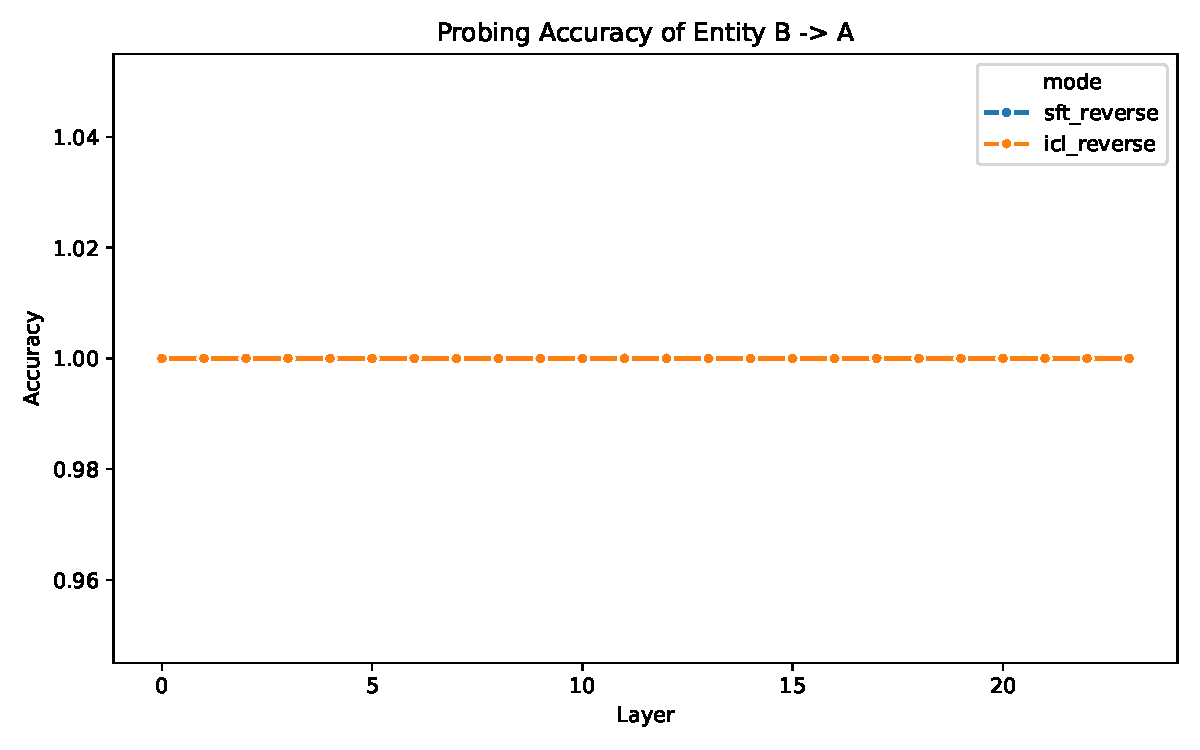
\includegraphics[width=0.7\textwidth]{figures/gpt2_medium/fig_appendix_probing.pdf}
\caption{Probing accuracy by layer for GPT-2 Medium (representative of all
three scales). All layers achieve 100\% training accuracy under both SFT and
ICL conditions, a consequence of high-dimensional geometry rather than
meaningful representational structure.}
\label{fig:figA_probing}
\end{figure}

\clearpage
\section{Full Activation Patching Results}
\label{app:patching}

\subsection{GPT-2 Medium}

\begin{figure}[h]
\centering
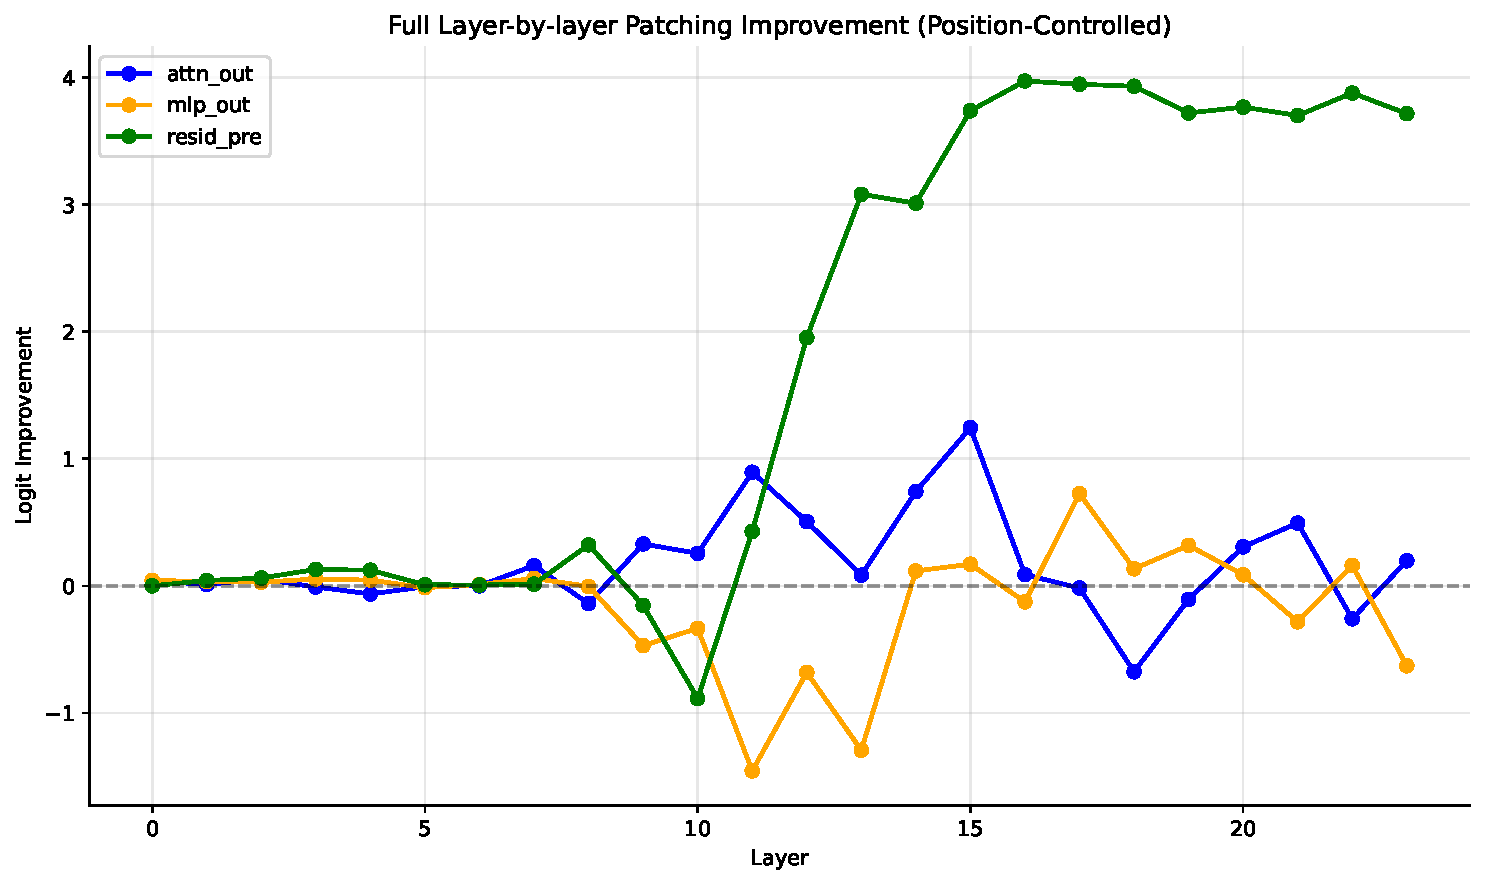
\includegraphics[width=0.8\textwidth]{figures/gpt2_medium/fig_S1.pdf}
\caption{Full layer-by-layer patching improvement for GPT-2 Medium across
all 24 layers and three component types (\texttt{resid\_pre}, \texttt{attn\_out},
\texttt{mlp\_out}).}
\label{fig:figS1}
\end{figure}

\begin{figure}[h]
\centering
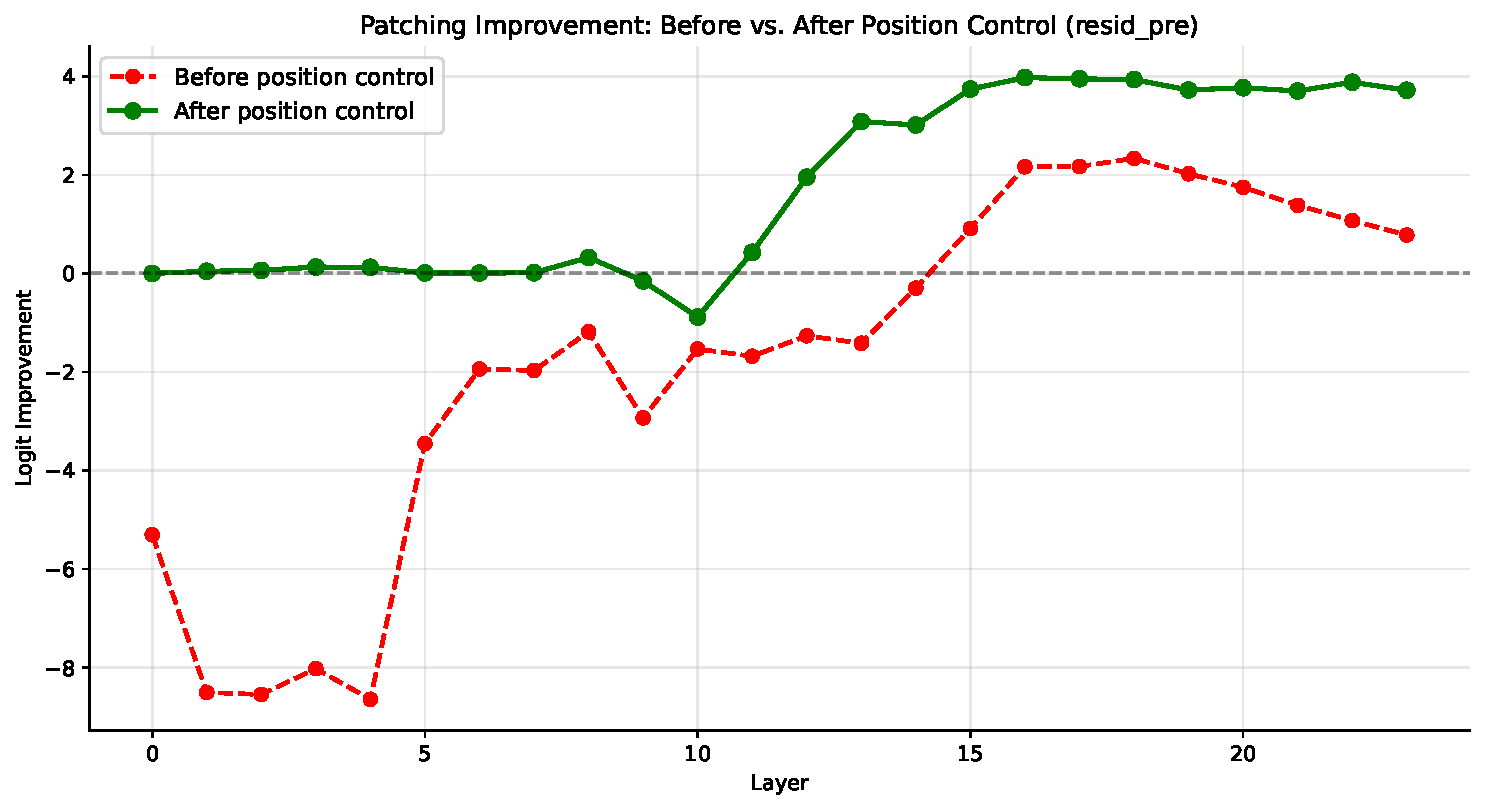
\includegraphics[width=0.8\textwidth]{figures/gpt2_medium/figS1_comparison.pdf}
\caption{Comparison of \texttt{resid\_pre} patching improvement before (red
dashed) and after (green solid) controlling for sequence-length mismatch,
GPT-2 Medium. The position-control eliminates artifactual early-layer
collapse.}
\label{fig:figS1b}
\end{figure}

\subsection{GPT-2 Small}
\label{app:smallpatching}

In GPT-2 Small (12 layers), the \texttt{resid\_pre} patching improvement rises
sharply from layer 7 onward, reaching a plateau at layers 10--11 with maximum
improvement of $+6.70$ and $+6.66$ respectively. Early layers (0--5) show
near-zero improvement ($< 0.20$). The relative location of the bottleneck
(upper two of twelve layers) is consistent with the Medium finding.

\begin{figure}[h]
\centering
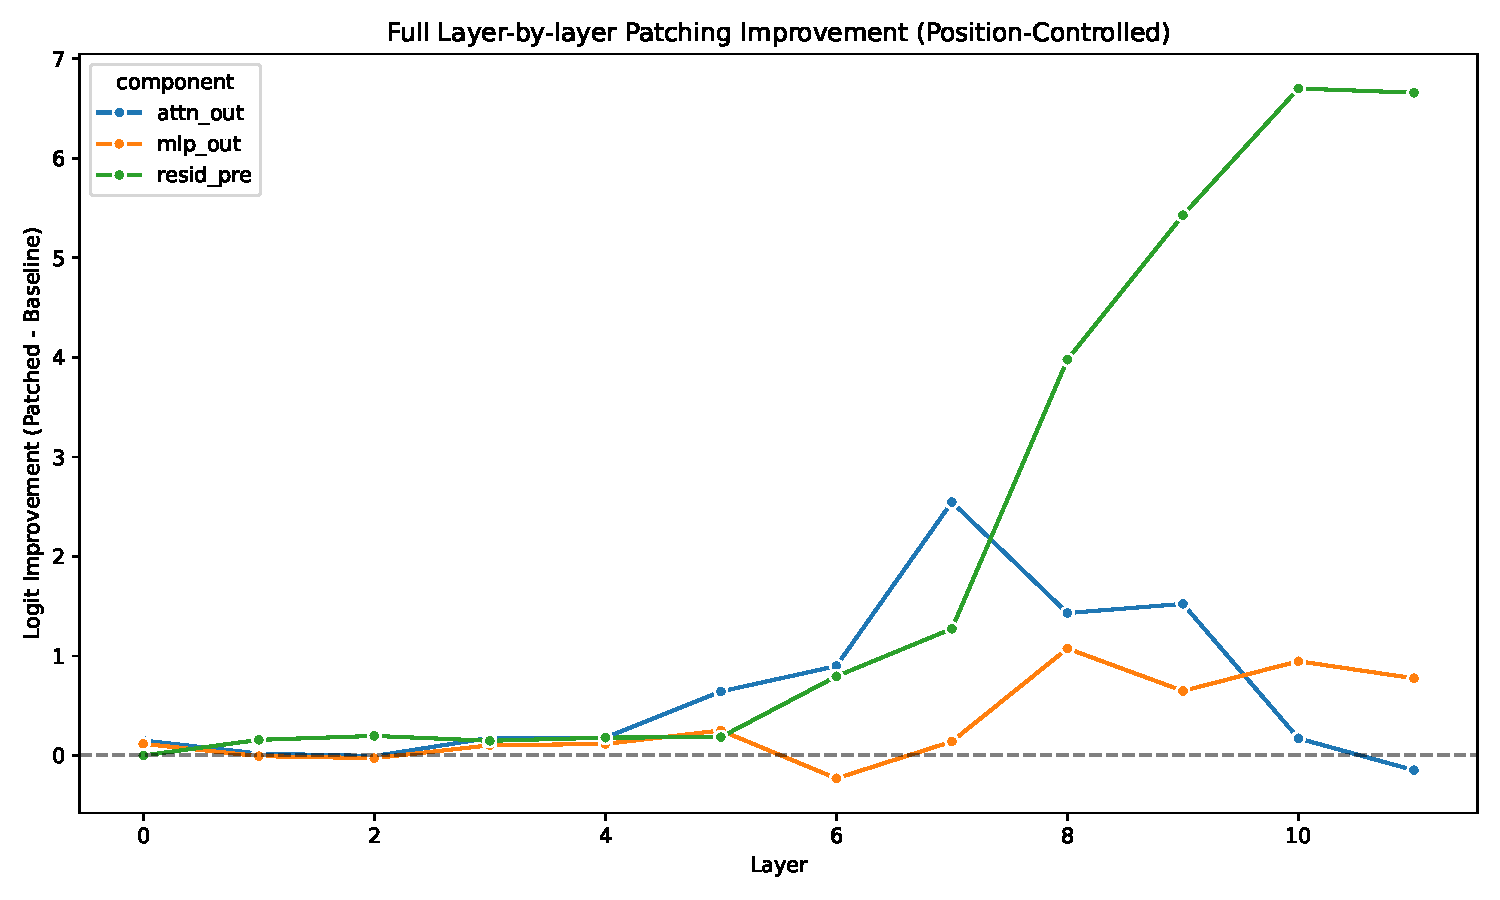
\includegraphics[width=0.8\textwidth]{figures/gpt2_small/fig_S1.pdf}
\caption{Full layer-by-layer patching improvement for GPT-2 Small across
all 12 layers and three component types.}
\label{fig:figS1_small}
\end{figure}

\subsection{GPT-2 Large}
\label{app:largepatching}

In GPT-2 Large (36 layers), the \texttt{resid\_pre} improvement rises steadily
from layer 10 onward, reaches a broad plateau from layers 22--35, and peaks
at layer 25 with improvement $+6.83$. Early layers (0--9) show minimal
improvement ($< 0.36$). The relative position of the plateau onset (layer 22
of 36, approximately the 61st percentile) closely matches the onset in Medium
(layer 16 of 24, approximately the 67th percentile).

\begin{figure}[h]
\centering
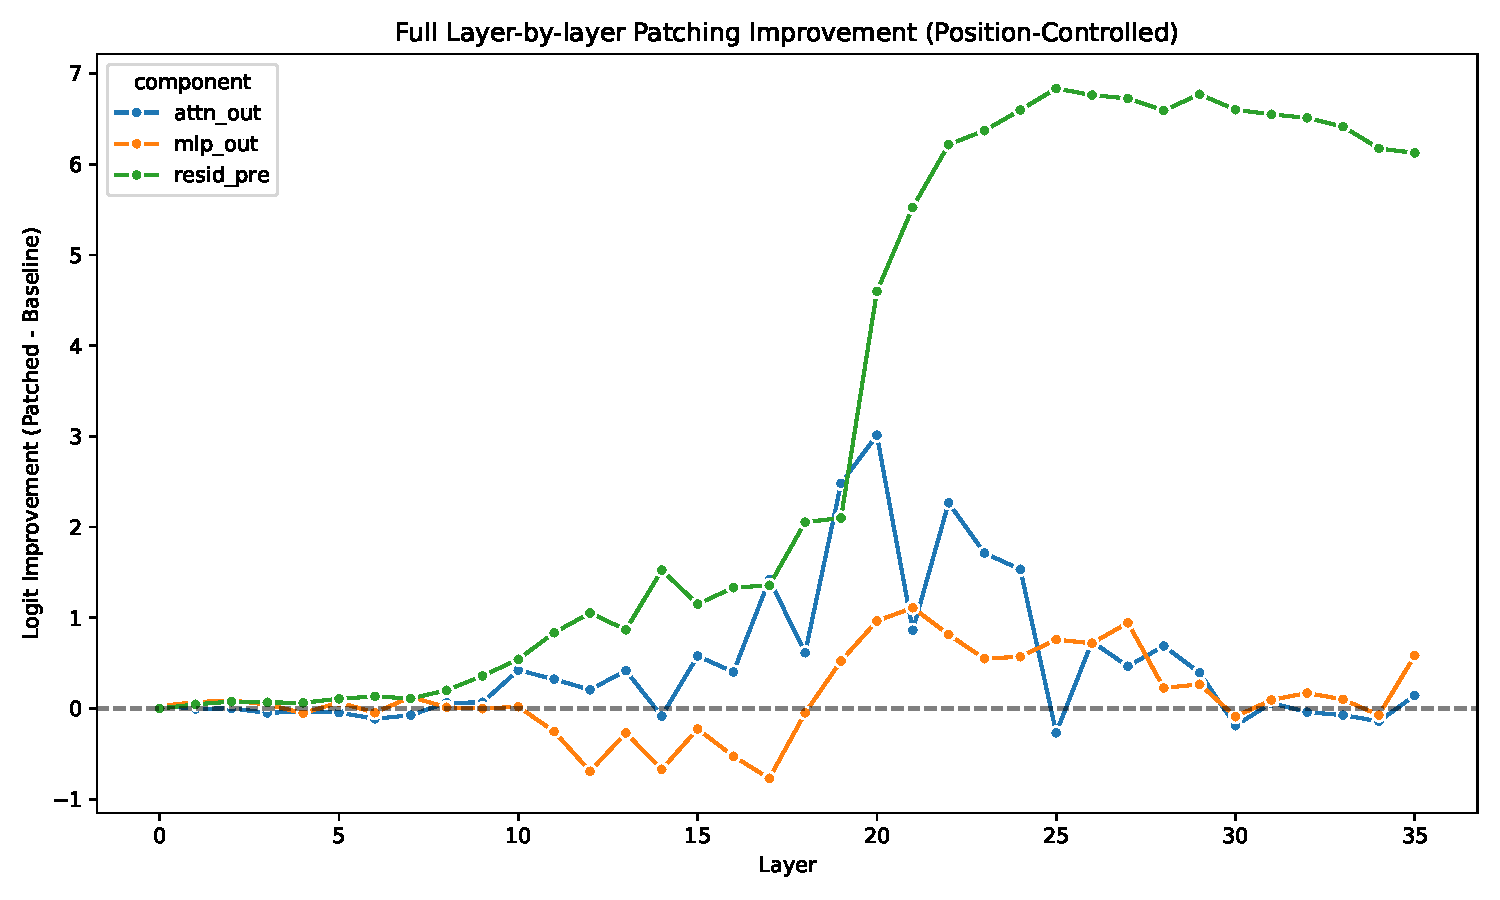
\includegraphics[width=0.8\textwidth]{figures/gpt2_large/fig_S1.pdf}
\caption{Full layer-by-layer patching improvement for GPT-2 Large across
all 36 layers and three component types.}
\label{fig:figS1_large}
\end{figure}

\clearpage
\section{Per-Relation-Type Breakdown}
\label{app:perrelation}

\subsection{GPT-2 Medium}

\begin{figure}[H]
\centering
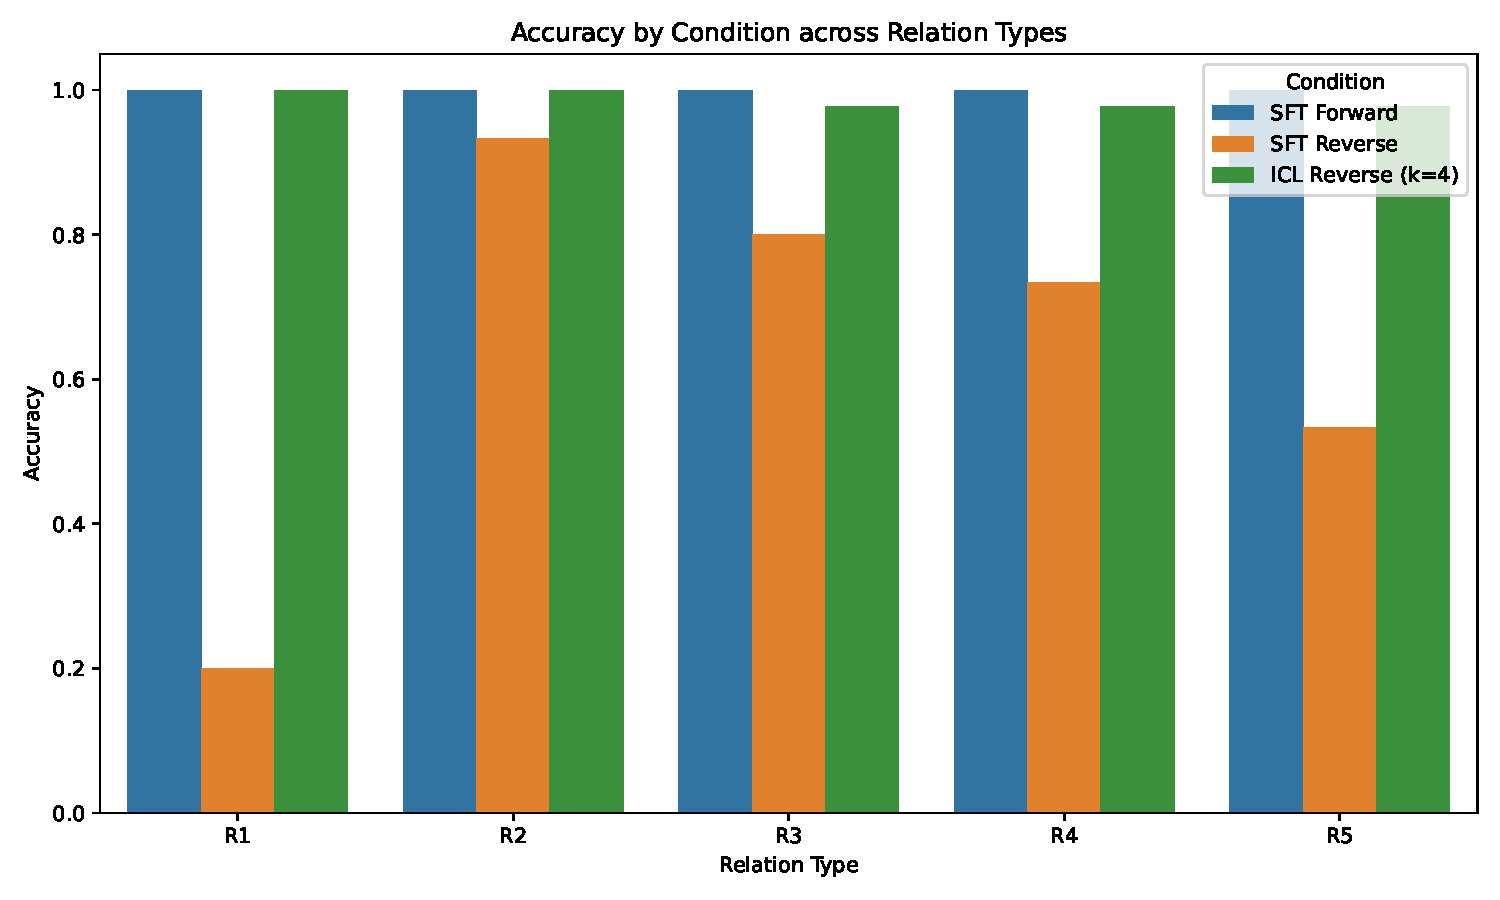
\includegraphics[width=0.8\textwidth]{figures/gpt2_medium/fig_S2.pdf}
\caption{Accuracy by condition (SFT Forward, SFT Reverse, ICL $k=4$ Reverse)
separately for each of the five relation types, GPT-2 Medium.}
\label{fig:figS2_medium}
\end{figure}

\begin{table}[H]
\centering
\caption{Accuracy by relation type, GPT-2 Medium.}
\label{tab:relation_acc_medium}
\begin{tabular}{lccc}
\toprule
\textbf{Relation} & \textbf{SFT Forward} & \textbf{SFT Reverse} & \textbf{ICL Reverse ($k=4$)} \\
\midrule
R1 & 100.00\% &  20.00\% & 100.00\% \\
R2 & 100.00\% &  93.33\% & 100.00\% \\
R3 & 100.00\% &  80.00\% &  97.78\% \\
R4 & 100.00\% &  73.33\% &  97.78\% \\
R5 & 100.00\% &  53.33\% &  97.78\% \\
\bottomrule
\end{tabular}
\end{table}

\subsection{GPT-2 Small and Large}

\begin{table}[H]
\centering
\caption{Accuracy by relation type, GPT-2 Small.}
\label{tab:relation_acc_small}
\begin{tabular}{lccc}
\toprule
\textbf{Relation} & \textbf{SFT Forward} & \textbf{SFT Reverse} & \textbf{ICL Reverse ($k=4$)} \\
\midrule
R1 & 100.00\% &   0.00\% & 100.00\% \\
R2 & 100.00\% &  20.00\% & 100.00\% \\
R3 & 100.00\% &   6.67\% &  86.67\% \\
R4 & 100.00\% &  20.00\% &  93.33\% \\
R5 & 100.00\% &   0.00\% &  97.78\% \\
\bottomrule
\end{tabular}
\end{table}

\begin{table}[H]
\centering
\caption{Accuracy by relation type, GPT-2 Large.}
\label{tab:relation_acc_large}
\begin{tabular}{lccc}
\toprule
\textbf{Relation} & \textbf{SFT Forward} & \textbf{SFT Reverse} & \textbf{ICL Reverse ($k=4$)} \\
\midrule
R1 & 100.00\% &   0.00\% & 100.00\% \\
R2 & 100.00\% &  46.67\% & 100.00\% \\
R3 & 100.00\% &  20.00\% & 100.00\% \\
R4 & 100.00\% &  53.33\% & 100.00\% \\
R5 & 100.00\% &  80.00\% & 100.00\% \\
\bottomrule
\end{tabular}
\end{table}

\section{Wrong-Label ICL Ablation}
\label{app:wronglabel}

As reported in Table~\ref{tab:main_results}, ICL with $k=4$ demonstrations
containing wrong constant-placeholder labels achieves 0.00\% accuracy at all
three model scales. In this implemented control, each demonstration's true
answer is replaced with the constant placeholder token \texttt{ZXQFVB},
guaranteeing no demonstration provides correct semantic content while preserving
the structural format of the prompt. This control confirms that ICL success
depends on correct semantic label content in demonstrations, not merely on
structurally matching the question prefix~\cite{min2022rethinking}.

\textbf{Note on legacy artifact (GPT-2 Medium only):} The repository also
contains \texttt{results/gpt2\_medium/tables/wrong\_label\_controls.csv}, which
averages to 5.78\% accuracy. The script that generated that file is not present
in the repository. The primary wrong-label control, generated by the maintained
pipeline in \texttt{src/icl/evaluate\_icl.py} with \texttt{---wrong-labels},
gives 0.00\%, and this is the result we report.

\section{Induction Head Verification}
\label{app:induction}

To verify whether the top-10 ICL-reverse DLA attention heads possess induction
head properties, we computed prefix-matching scores on random repeated-token
sequences (128 sequences, prefix length 32, threshold $> 0.40$).

\subsection{GPT-2 Medium}

\begin{table}[H]
\centering
\caption{Prefix-matching induction scores for the top-10 DLA heads,
GPT-2 Medium. A score $>0.40$ is the standard threshold for induction heads.}
\label{tab:induction_medium}
\begin{tabular}{ccc}
\toprule
\textbf{Layer} & \textbf{Head} & \textbf{Induction Score} \\
\midrule
18 &  5 & 0.950 \\
20 & 12 & 0.869 \\
19 & 15 & 0.786 \\
20 &  7 & 0.711 \\
16 & 15 & 0.466 \\
18 & 12 & 0.223 \\
15 & 14 & 0.138 \\
23 &  6 & 0.108 \\
20 &  4 & 0.069 \\
14 & 14 & 0.008 \\
\bottomrule
\end{tabular}
\end{table}

Five of the ten top-DLA heads pass the induction threshold (0.466--0.950). Note
that these are the high-magnitude late-layer ``final-write'' heads, not the
early-to-mid layers 6, 7, 9--11, 13--15 identified as dissociation-specific in
Section~\ref{sec:dla}. Whether the dissociation-specific population also exhibits
induction properties is an open question for future work.

\subsection{GPT-2 Small}

\begin{table}[H]
\centering
\caption{Prefix-matching induction scores for the top-10 DLA heads,
GPT-2 Small.}
\label{tab:induction_small}
\begin{tabular}{cccc}
\toprule
\textbf{Rank} & \textbf{Layer} & \textbf{Head} & \textbf{Induction Score} \\
\midrule
1  & 10 & 10 & 0.253 \\
2  &  9 &  9 & 0.603 \\
3  &  9 &  6 & 0.588 \\
4  &  8 & 11 & 0.011 \\
5  & 10 &  0 & 0.479 \\
6  & 10 &  1 & 0.587 \\
7  & 11 &  8 & 0.014 \\
8  &  7 & 11 & 0.058 \\
9  &  8 &  3 & 0.072 \\
10 &  6 &  9 & 0.940 \\
\bottomrule
\end{tabular}
\end{table}

Five of ten top-DLA heads in Small also pass the induction threshold (scores:
0.603, 0.588, 0.479, 0.587, 0.940 for ranks 2, 3, 5, 6, 10 respectively).

\subsection{GPT-2 Large}

\begin{table}[H]
\centering
\caption{Prefix-matching induction scores for the top-10 DLA heads,
GPT-2 Large.}
\label{tab:induction_large}
\begin{tabular}{cccc}
\toprule
\textbf{Rank} & \textbf{Layer} & \textbf{Head} & \textbf{Induction Score} \\
\midrule
1  & 23 &  7 & 0.164 \\
2  & 29 &  1 & 0.034 \\
3  & 22 &  0 & 0.190 \\
4  & 26 &  3 & 0.445 \\
5  & 27 & 17 & 0.732 \\
6  & 30 & 11 & 0.034 \\
7  & 24 & 13 & 0.381 \\
8  & 27 & 12 & 0.271 \\
9  & 30 & 10 & 0.229 \\
10 & 24 &  5 & 0.149 \\
\bottomrule
\end{tabular}
\end{table}

Only 2 of the 10 top-DLA heads in Large pass the induction threshold (Layer 26,
Head 3: score 0.445; Layer 27, Head 17: score 0.732). This is substantially
fewer than in Small or Medium (5/10 each), consistent with the observation that
the high-DLA heads in Large operate via less induction-like mechanisms.

\clearpage
\section{GPT-2 Large Behavioral and Mechanistic Figures}
\label{app:largefigs}

\begin{figure}[H]
\centering
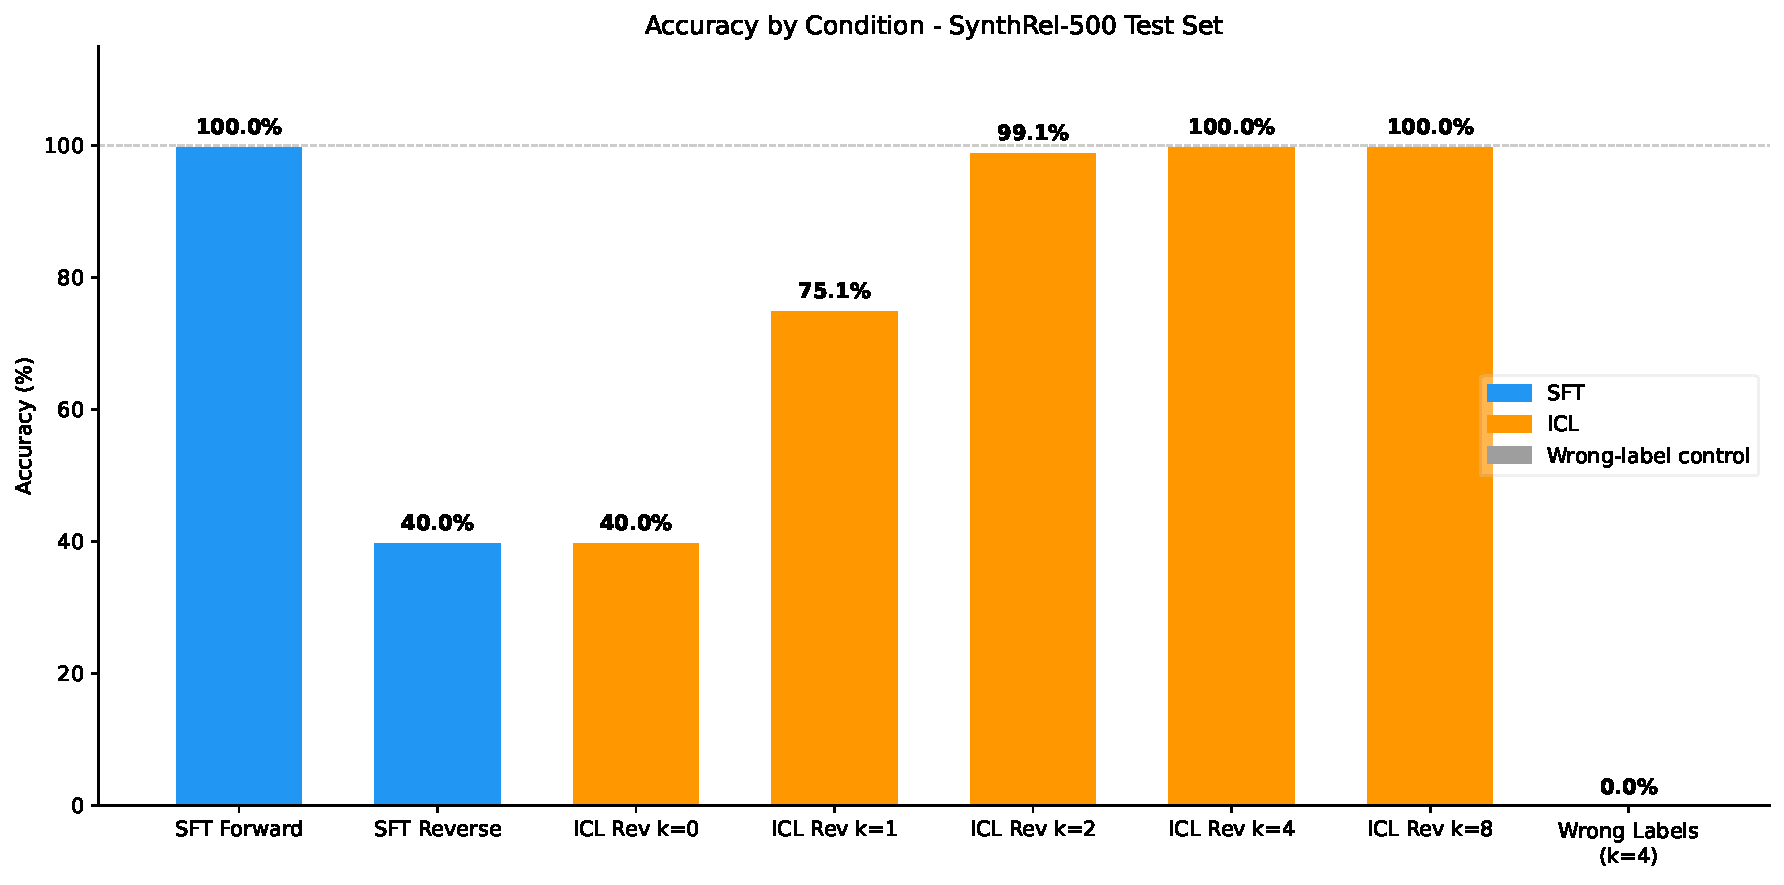
\includegraphics[width=0.8\textwidth]{figures/gpt2_large/fig1.pdf}
\caption{Bar chart of primary accuracy conditions for GPT-2 Large.}
\label{fig:fig1_large}
\end{figure}

\begin{figure}[H]
\centering
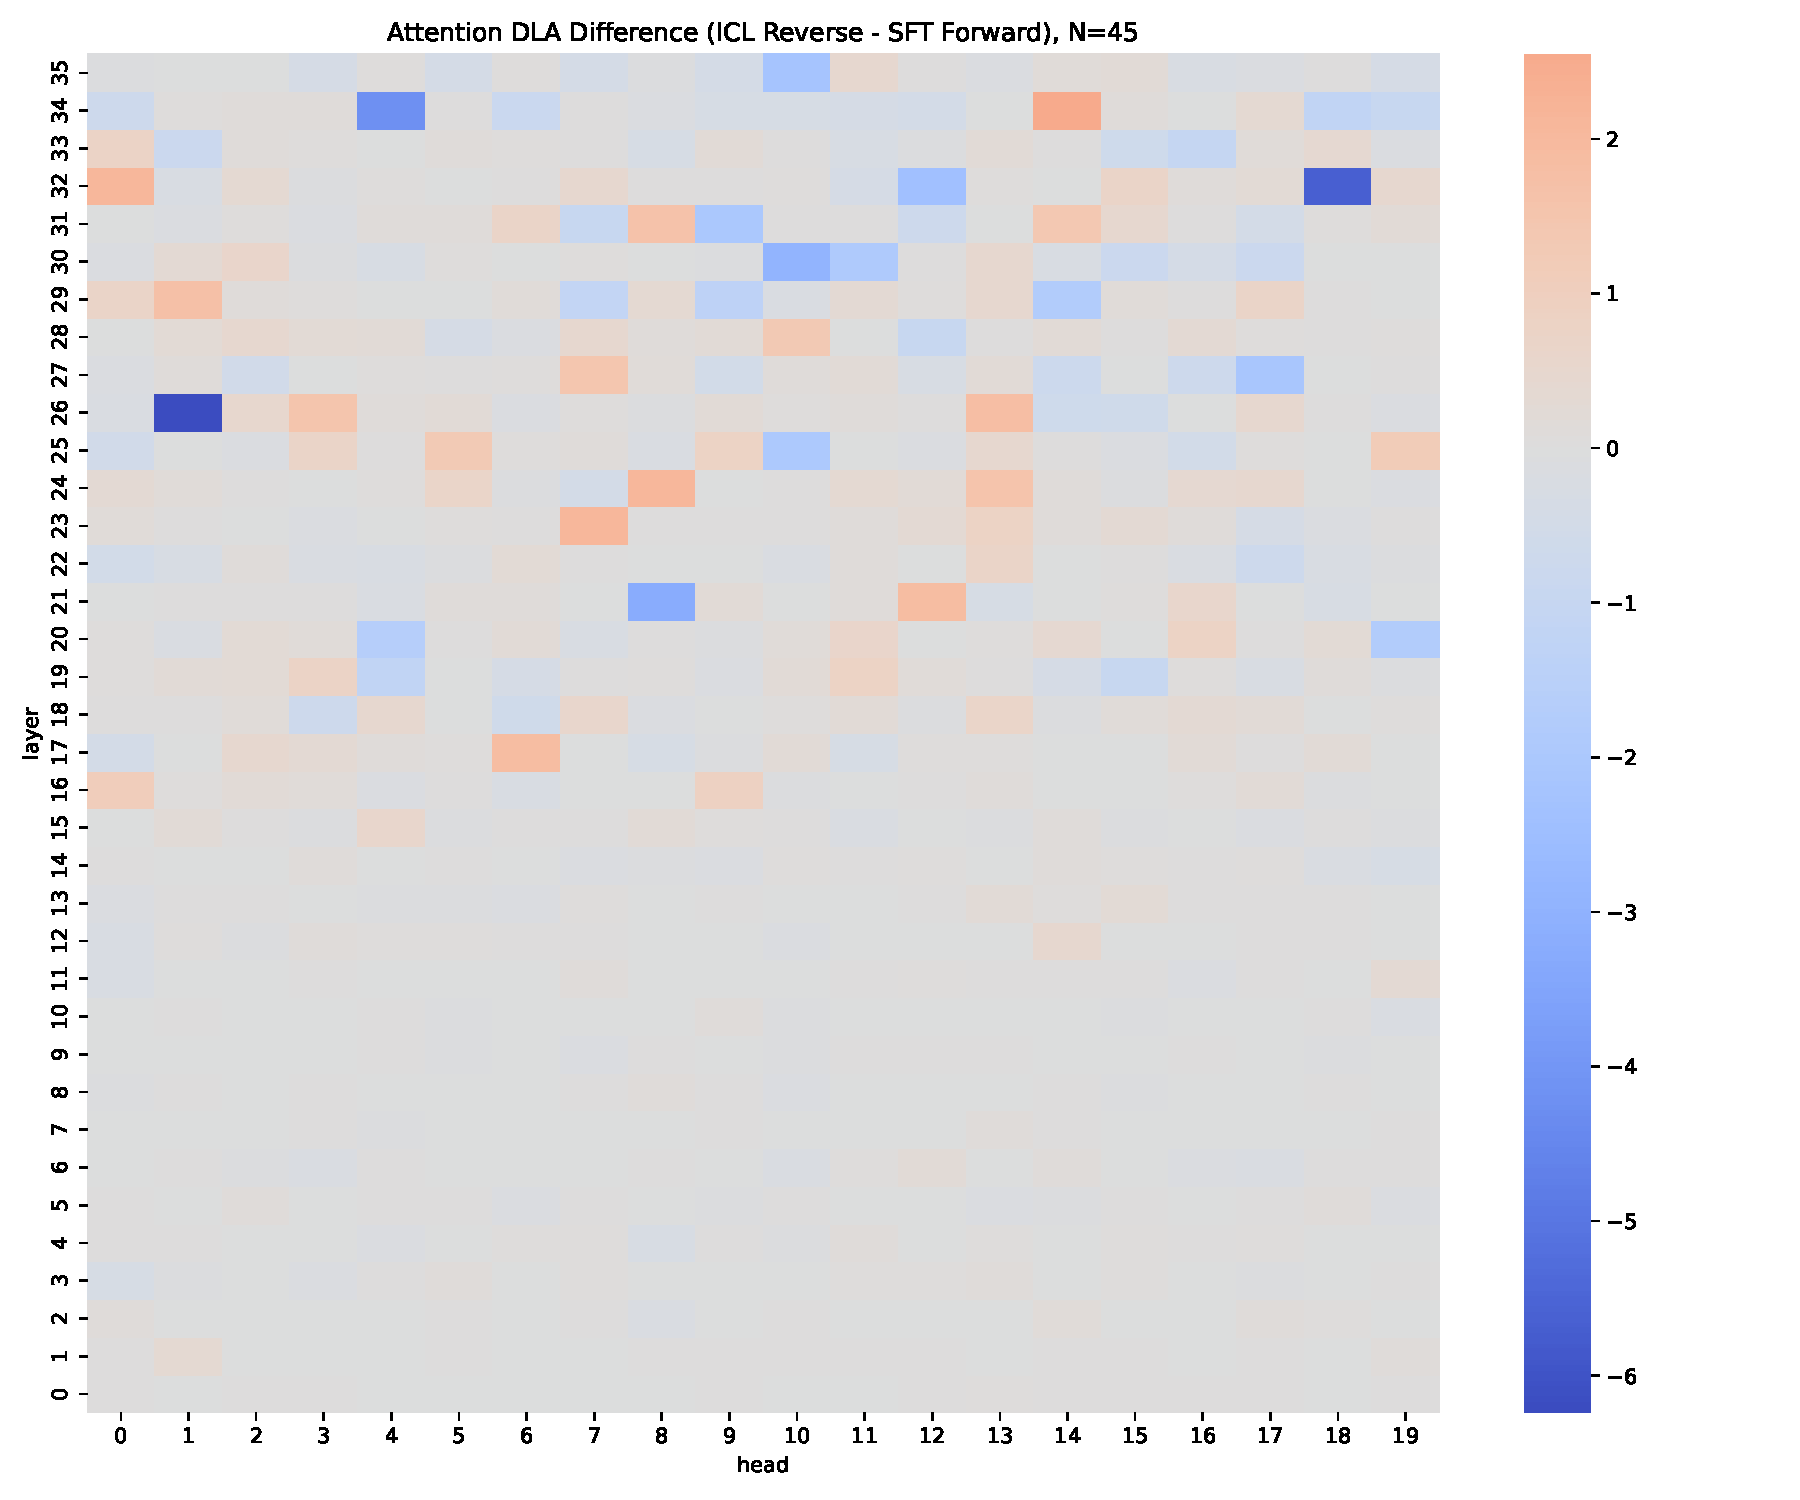
\includegraphics[width=0.8\textwidth]{figures/gpt2_large/fig4a.pdf}
\caption{DLA heatmap (attention heads) for ICL reverse vs.\ SFT forward,
GPT-2 Large ($N=45$ eligible items).}
\label{fig:fig4_large}
\end{figure}

\begin{figure}[H]
\centering
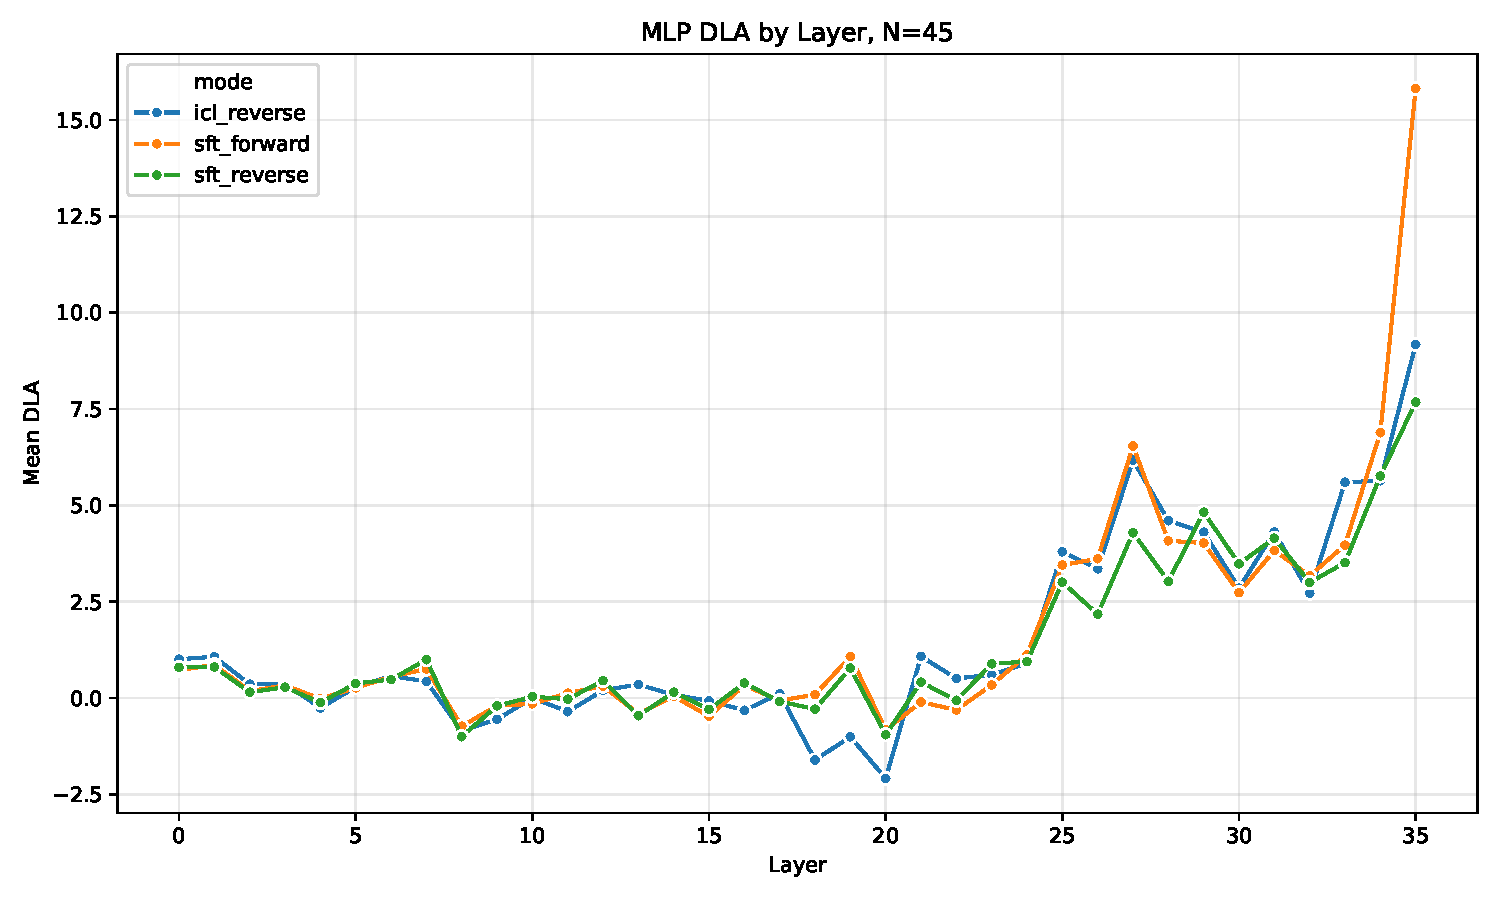
\includegraphics[width=0.8\textwidth]{figures/gpt2_large/fig4b.pdf}
\caption{MLP DLA by layer for three conditions, GPT-2 Large.}
\label{fig:fig4b_large}
\end{figure}

\begin{figure}[H]
\centering
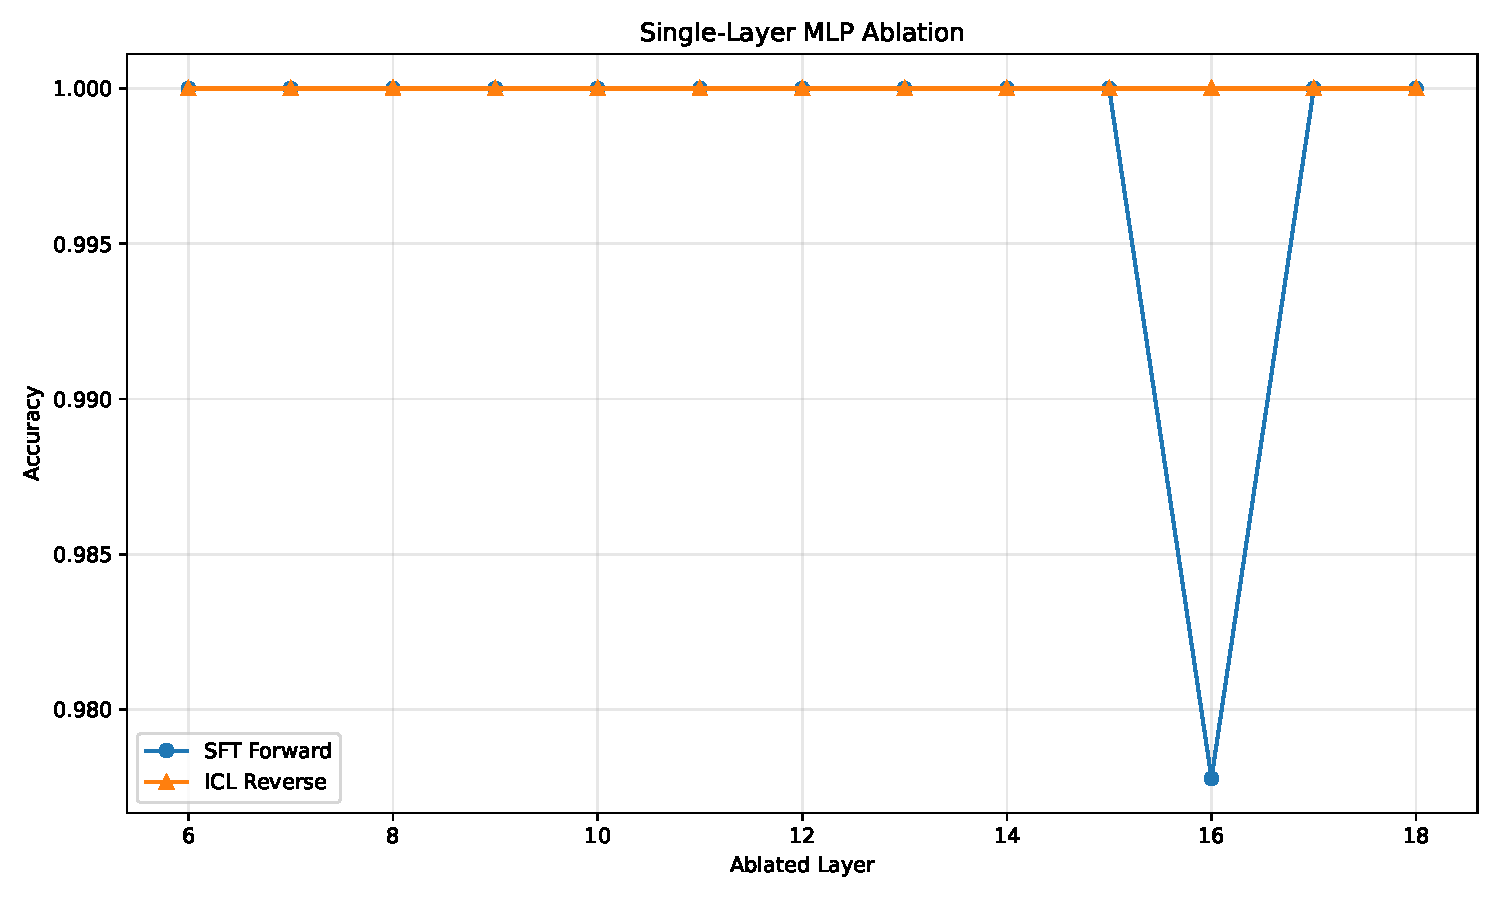
\includegraphics[width=0.8\textwidth]{figures/gpt2_large/fig5.pdf}
\caption{Single-layer MLP ablation sweep, GPT-2 Large. ICL reverse
accuracy remains at 100\% across all ablated layers; SFT forward drops by
2.2\% only at layer 16.}
\label{fig:fig5_large}
\end{figure}

\section{GPT-2 Small Behavioral and Mechanistic Figures}
\label{app:smallfigs}

\begin{figure}[H]
\centering
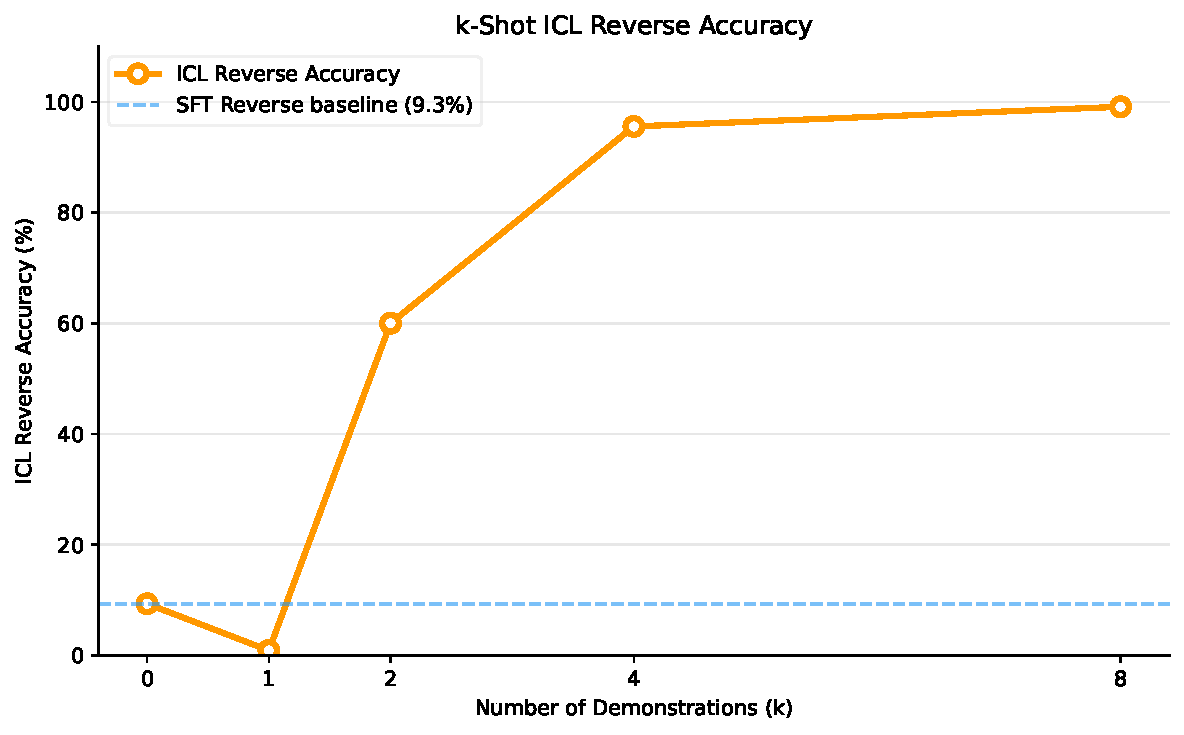
\includegraphics[width=0.6\textwidth]{figures/gpt2_small/fig2.pdf}
\caption{$k$-shot accuracy curve for GPT-2 Small. The $k=1$ interference trough
is pronounced (0.89\%), consistent with the Medium pattern and contrasting with
Large's improvement at $k=1$.}
\label{fig:fig2_small}
\end{figure}

\begin{figure}[H]
\centering
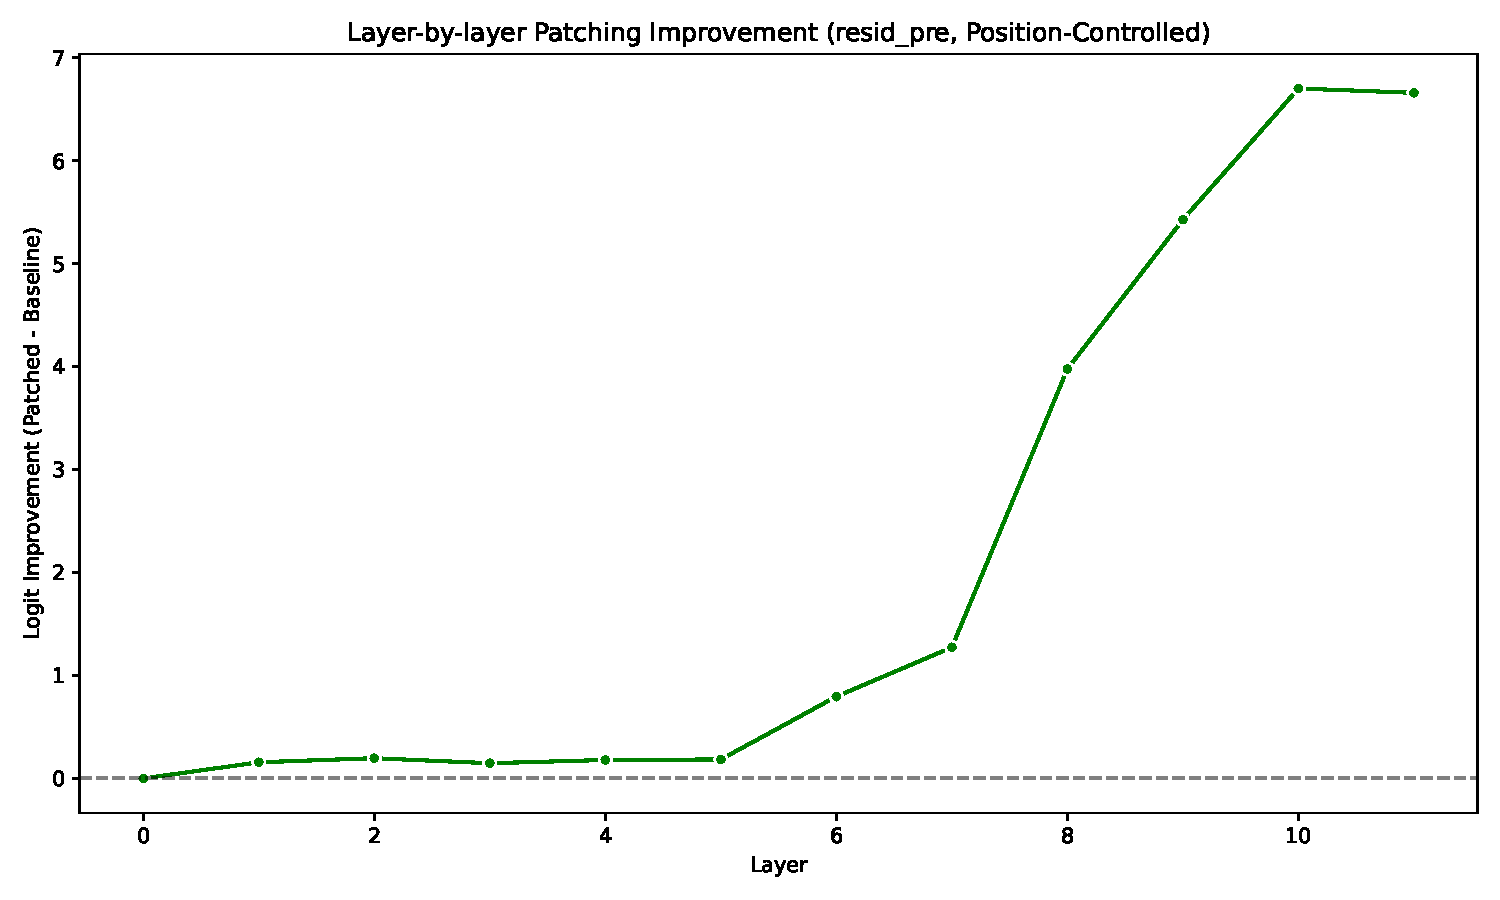
\includegraphics[width=0.8\textwidth]{figures/gpt2_small/fig3.pdf}
\caption{Layer-by-layer patching improvement (resid\_pre) for GPT-2
Small. The bottleneck appears at layers 10--11 (the top two of twelve layers).}
\label{fig:fig3_small}
\end{figure}

\begin{figure}[H]
\centering
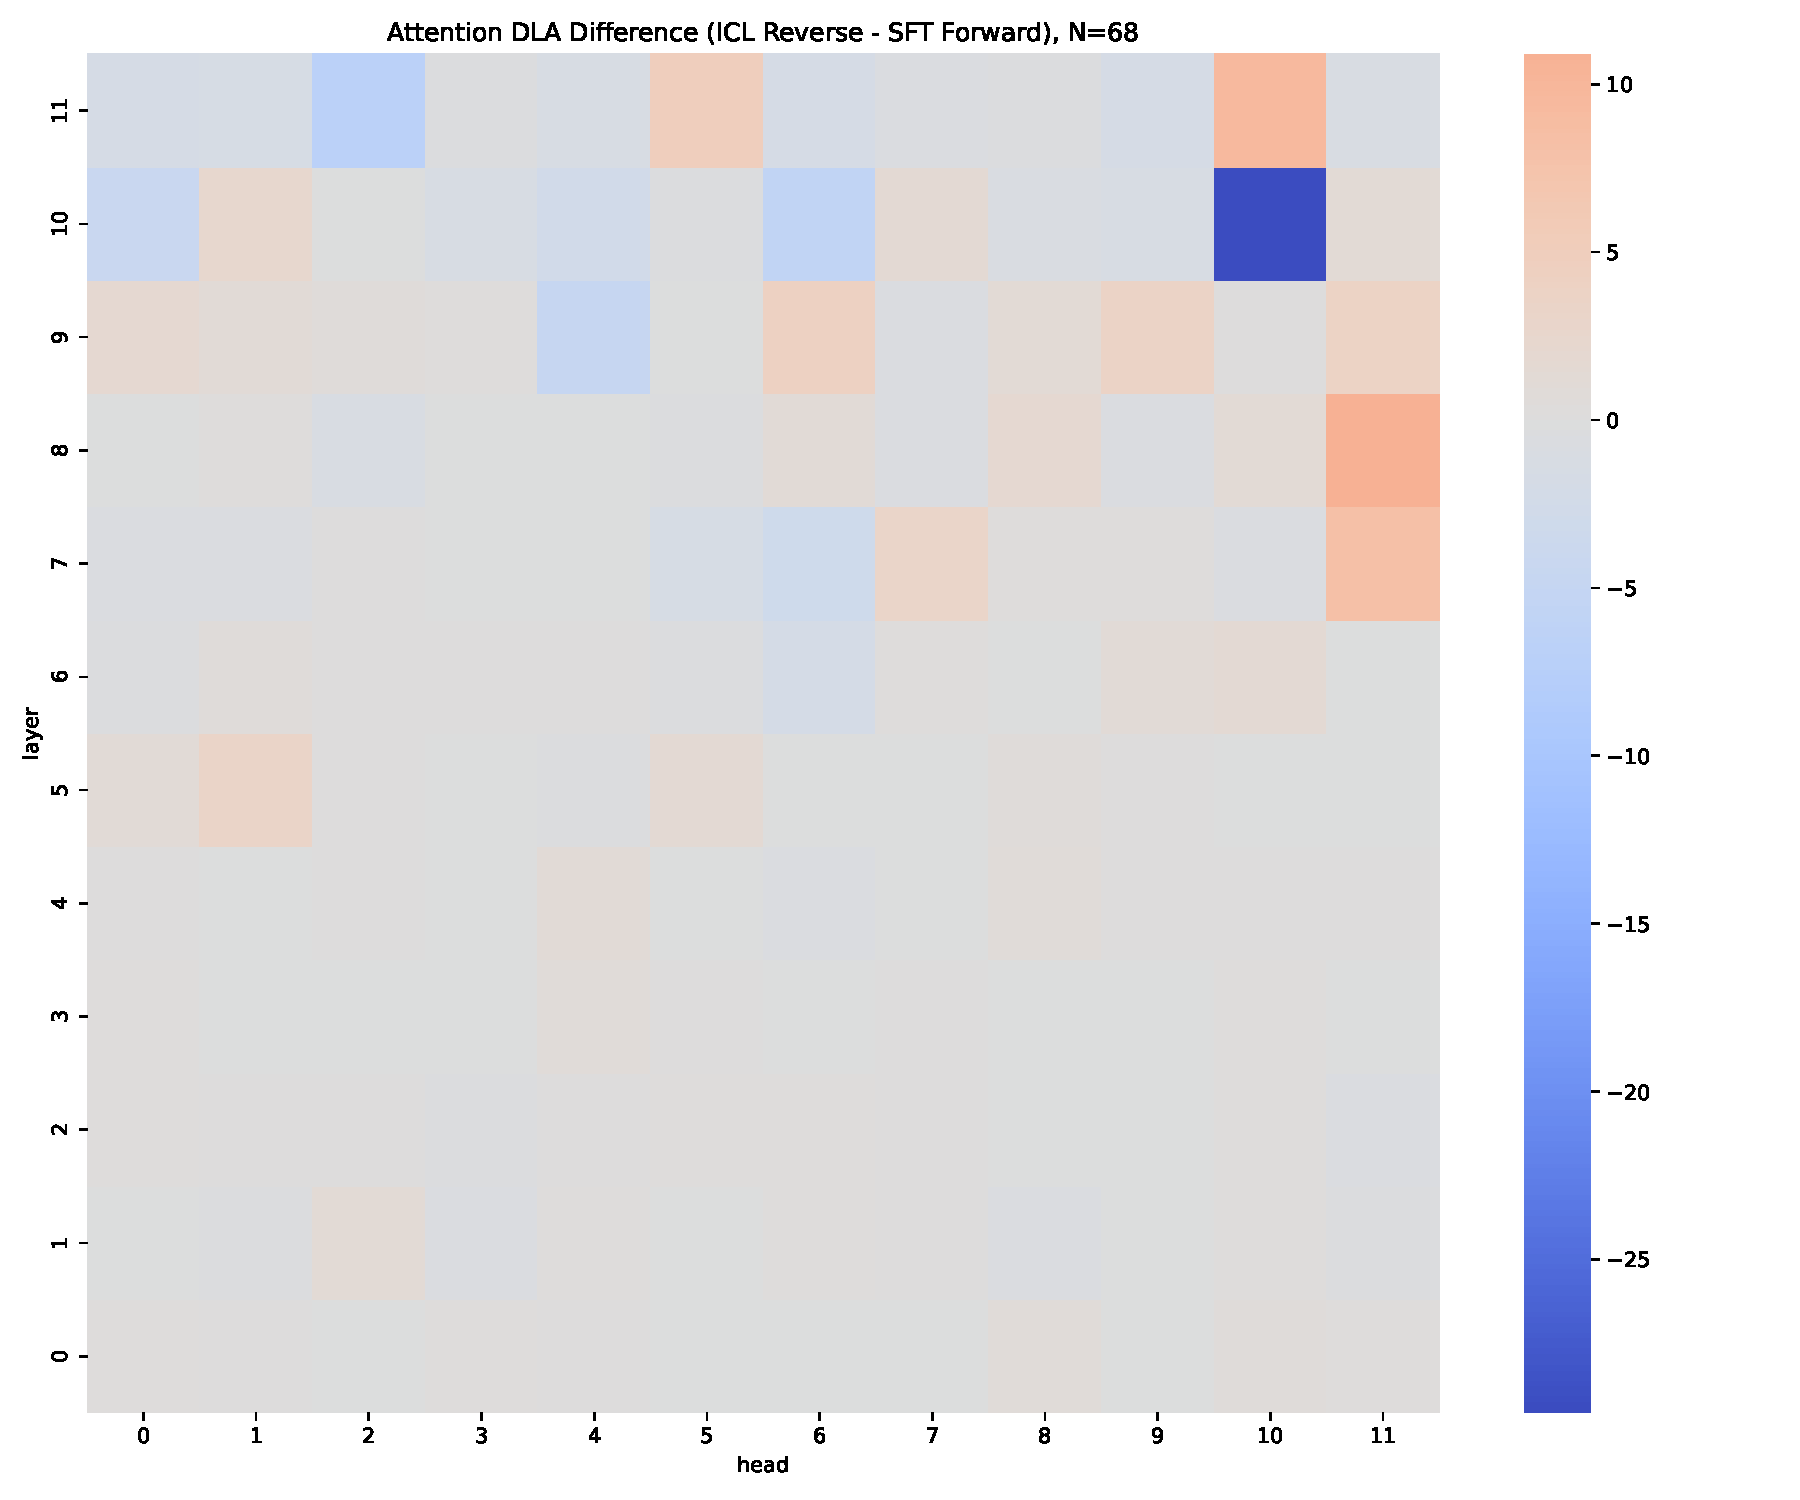
\includegraphics[width=0.8\textwidth]{figures/gpt2_small/fig4a.pdf}
\caption{DLA heatmap (attention heads) for ICL reverse vs.\ SFT forward,
GPT-2 Small ($N=68$ eligible items).}
\label{fig:fig4_small}
\end{figure}

\begin{figure}[H]
\centering
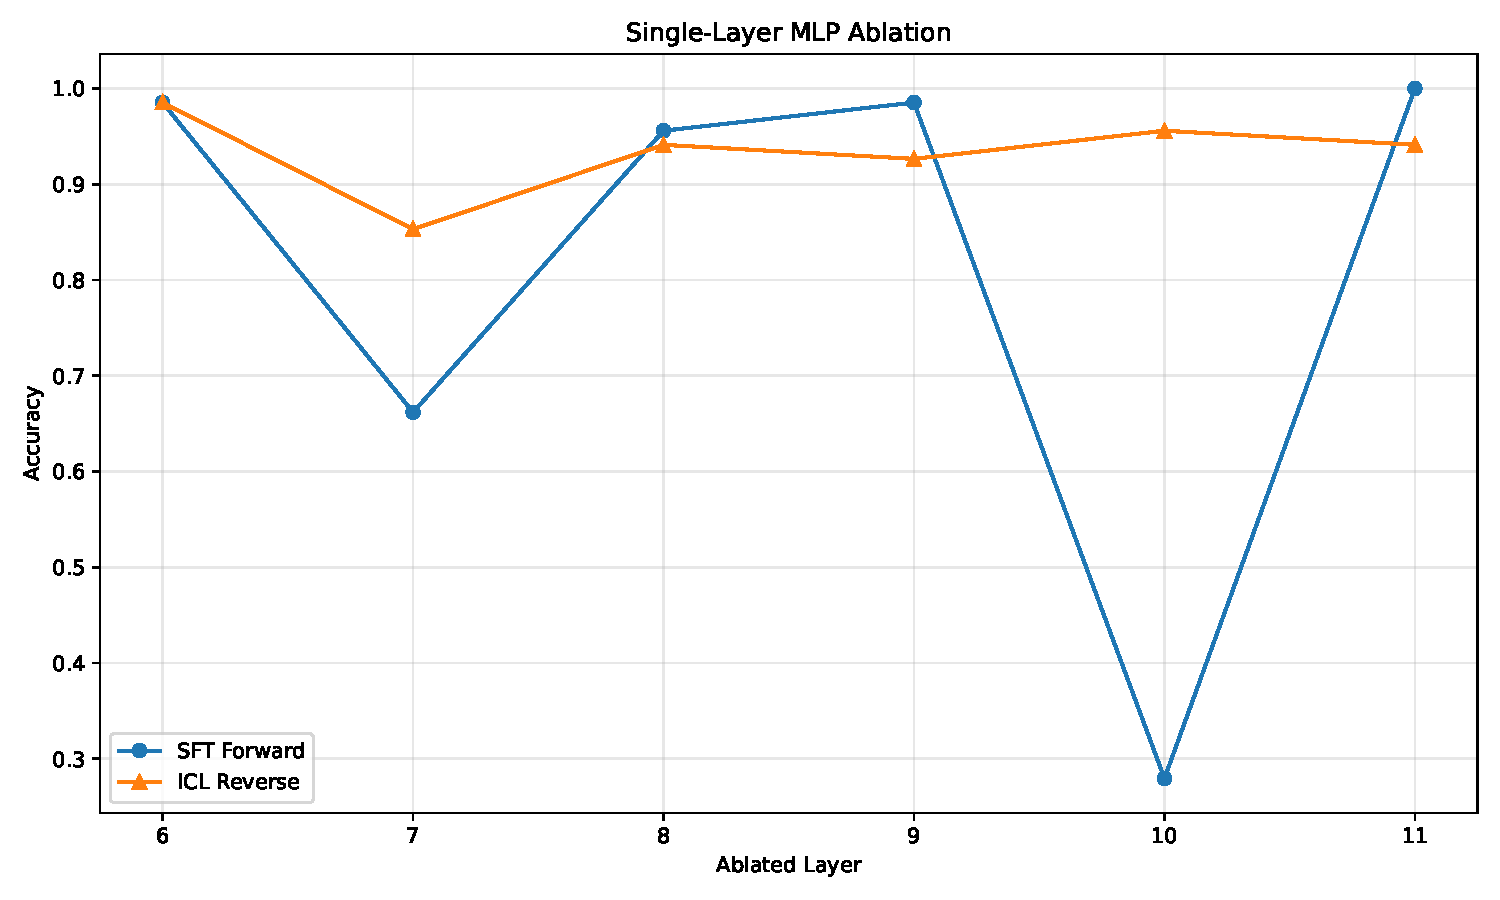
\includegraphics[width=0.8\textwidth]{figures/gpt2_small/fig5.pdf}
\caption{Single-layer MLP ablation sweep, GPT-2 Small. Layer 10 produces a
large drop in SFT forward accuracy (72.1\%); ICL reverse accuracy remains
nearly stable across all layers.}
\label{fig:fig5_small}
\end{figure}

\clearpage
\section{Statistical Reporting Notes}
\label{app:stats}

All behavioral $p$-values in the main text are reported as raw, uncorrected
values for the primary confirmatory hypotheses (SFT forward vs.\ reverse;
ICL $k=4$ reverse vs.\ SFT reverse). For the full DLA layer-level analysis,
Benjamini-Hochberg FDR correction is applied within each model's test family
(as reported in Tables~\ref{tab:dla_sig} and~\ref{tab:dla_sig_mlp}). The full
set of raw and corrected $p$-values is released in the supplementary data
repository for independent verification.

Cohen's $d$ for the SFT forward vs.\ reverse comparisons is computed from
paired binary item-level scores. For ICL $k=4$ reverse vs.\ SFT reverse, a
Wilcoxon signed-rank test is used because ICL item-level scores are continuous
per-item mean-correct values averaged over three demonstration samplings, not
binary.

Confidence intervals are computed via 10,000-iteration item bootstrap (percentile
method, seed 42).

\section{Technical Implementation Notes}
\label{app:technical}

We document the following library-level adjustments from the initial
experimental design, for reproduction purposes:

\begin{itemize}
  \item \texttt{TrainingArguments} parameter renamed from
  \texttt{evaluation\_strategy} to \texttt{eval\_strategy} in
  \texttt{transformers} $\geq$ 4.41.

  \item TransformerLens does not cache \texttt{hook\_result} by default
  (memory optimization). Per-head attribution was computed via
  $\hat{z}_h = z_h W_O^h$ using \texttt{einsum}, where $z_h$ is the cached
  \texttt{hook\_z} output and $W_O^h$ is the head's output projection matrix.
  This is mathematically equivalent.

  \item \texttt{LogisticRegression(multi\_class=``multinomial'')} deprecated
  in \texttt{scikit-learn} $\geq$ 1.5; the argument was removed.

  \item Entity names are sometimes tokenized into multiple subword tokens.
  In activation analysis scripts, we use the first token of each entity
  name as the target position.

  \item An earlier single-layer MLP ablation sweep incorrectly evaluated SFT
  accuracy against \texttt{reverse\_question} prompts instead of
  \texttt{forward\_question} prompts. A separate earlier evaluation-loop error
  in the attention-head ablation script used out-of-relation training examples
  as $k$-shot demonstrations. Both errors were identified and corrected prior to
  the results reported in this paper.

  \item The epoch ablation artifact \texttt{eval\_final\_model.csv} evaluates
  the same checkpoint as \texttt{eval\_sft\_finetuned.csv} but is generated
  independently by the robustness pipeline; small numerical differences between
  them reflect different evaluation randomness, not different model weights.
  All primary reported statistics use \texttt{eval\_sft\_finetuned.csv}.
\end{itemize}

All code, data, and checkpoints are released at
\url{https://github.com/AA-KH/Reversal-Curse-Mechanisms.git}.

\end{document}
